\documentclass{article}
% \usepackage[nonatbib]{neurips_2022}
\PassOptionsToPackage{numbers, compress}{natbib}
% \PassOptionsToPackage{compress, numbers}{natbib}
\usepackage[final]{neurips_2022}
\usepackage[utf8]{inputenc} % allow utf-8 input
\usepackage[T1]{fontenc}    % use 8-bit T1 fonts
\usepackage{hyperref}       % hyperlinks
\usepackage{url}            % simple URL typesetting
\usepackage{booktabs}       % professional-quality tables
\usepackage{amsfonts}       % blackboard math symbols
\usepackage{nicefrac}       % compact symbols for 1/2, etc.
\usepackage{microtype}      % microtypography
\usepackage{xcolor}         % colors
\usepackage{graphicx}
\usepackage{comment}
\usepackage{amsmath,amssymb}
\usepackage{subfigure}
\usepackage[linesnumbered,ruled]{algorithm2e}
\usepackage{multirow}
\usepackage{nth}
\usepackage{amsthm}
\newtheorem{lemma}{Lemma}
\usepackage{adjustbox}
\usepackage[normalem]{ulem}
\usepackage{wrapfig,lipsum}
\usepackage{pgf-pie} 
\usepackage{multicol}
\usepackage{siunitx}

\newcommand{\rebuttal}[1]{\textcolor{black}{#1}}
\newcommand{\Luyang}[1]{\textcolor{orange}{(Luyang: #1)}}
\newcommand{\Samiul}[1]{\textcolor{blue}{#1}}

\newcommand{\MZ}[1]{\textcolor{red}{(MZ: #1)}}


%\title{Federated Learning of Heterogeneous Models with Scheduled Architecture Rolling}
\title{FedRolex: Model-Heterogeneous Federated Learning with Rolling Sub-Model Extraction}

%\begin{comment}
\author{
    Samiul Alam$^{1,2}$, Luyang Liu$^3$, Ming Yan$^{4,1}$, Mi Zhang$^{2,1}$\\
    \quad $^1$Michigan State University, $^2$The Ohio State University, \\\quad $^3$Google Research, \quad $^4$The Chinese University of Hong Kong, Shenzhen \\
    %{\small\texttt{zhengy30@msu.edu, zhiz@amazon.com, \{yanshen6, mizhang\}@msu.edu}}
    {\small\texttt{alamsami@msu.edu, luyangliu@google.com, yanming@cuhk.edu.cn, mizhang.1@osu.edu}}
}
%\end{comment}


\begin{document}

%% CR is 10 pages
\maketitle
\begin{abstract}


%% 1. Background.
%Federated learning (FL) is a privacy-preserving machine learning paradigm that trains a machine learning model on a federation of distributed clients while keeping their data locally.  %The process can be formulated as solving an optimization problem under constraint of minimizing communication overhead while ensuring robustness of model with heterogeneous data and privacy. However, in practical settings, even these constraints can be an oversimplification.
%%
%% 2. Limitations of existing works.
Most cross-device federated learning (FL) studies focus on the model-homogeneous setting where the global server model and local client models are identical. However, such constraint not only excludes low-end clients who would otherwise make unique contributions to model training but also restrains clients from training large models due to on-device resource bottlenecks.
%
%However, in real-world scenarios, such a requirement acts as a constraint that restricts the outreach to clients with heterogeneous device resources and unfairly excludes users with low-end devices who would otherwise benefit from FL. 
%Most FL research focus on training a single global model with the assumption of data heterogeneity. But in practical scenarios, the edge devices in the systems where these algorithms would be deployed will have vastly different compute capabilities. Having the same model deployed on all devices will restrict the outreach of the system and unfairly deprive low-end device users of the benefits of FL. It is therefore important to also optimize for model heterogeneity. 
%%
%% 3. Overview of our method: the key problem it addresses and its key techniques.
In this work, we propose \texttt{FedRolex}, a partial training (PT)-based approach that enables model-heterogeneous FL and can train a global server model larger than the largest client model. At its core, \texttt{FedRolex} employs a rolling sub-model extraction scheme that allows different parts of the global server model to be evenly trained, which mitigates the client drift induced by the inconsistency between individual client models and server model architectures. 
%\Luyang{Reorder this following part a bit, PTAL.}
% We provide a theoretical statistical analysis on its advantage over Federated Dropout. 
%
%Unlike the model-homogeneous scenario, the fundamental challenge of model heterogeneity in FL is that different parts of the global model are trained on heterogeneous data distributions. Our method addresses this challenge by rolling the sub-model in each federated iteration so that the parameters of the global model are evenly trained on the global data distribution across all devices.
%making it more akin to model-homogeneous training.
%Cognizant of the data heterogeneity property of FL,  
% However, model heterogeneity raises a key issue concerning optimal knowledge distillation. Unlike the homogeneous scenario, different parts of the global model are essentially trained on heterogeneous data distributions. 
% to distill knowledge evenly throughout the global model by rolling the model in every round so that all parts of the model see the entire data distribution making it more akin to homogeneous training.
%%
%% 4. Summary of our experiments and results.
%Empirically, 
We show that \texttt{FedRolex} outperforms state-of-the-art PT-based model-heterogeneous FL methods (e.g. Federated Dropout) and reduces the gap between model-heterogeneous and model-homogeneous FL, especially under the large-model large-dataset regime. In addition, we provide theoretical statistical analysis on its advantage over Federated Dropout and evaluate \texttt{FedRolex} on an emulated real-world device distribution to show that \texttt{FedRolex} can enhance the inclusiveness of FL and boost the performance of low-end devices that would otherwise not benefit from FL.
%we consider the distribution of client capabilities similar to real-world income distribution. Our results consistently improve the accuracy of low-end devices, which enhances the inclusiveness of federated learning.
%We evaluate our method with image classification and language modelling tasks using ResNet and Transformer models respectively. We also perform several ablation studies comparing performance to homogeneous setting, the accuracy of the algorithm in a real world model capacity distribution and the effect of the size of the global server model.
%which considerably enhances the inclusiveness of FL
%
Our code is available at: \href{https://github.com/AIoT-MLSys-Lab/FedRolex}{https://github.com/AIoT-MLSys-Lab/FedRolex}.
\end{abstract}


\section{Introduction} \label{intro}
\vspace{-1mm}

%\Luyang{We should cite \cite{wang2021field} somewhere.}

% P1: Brief background of FL: 2-3 sentences. Most existing works focus on model homogeneity. Talk about its limitations.
Federated learning (FL) is a machine learning paradigm that trains models from distributed clients with private data under the coordination of a central server \cite{kairouz2021advances, wang2021field}. In this work, we focus on cross-device FL where clients are usually resource-constrained edge devices.
%This idea has far-reaching applications and is made urgent by modern demands for privacy. 
%Indeed, the goal of strong data privacy is a central motivation for FL. By storing data locally, instead of replicating them on a remote server, the system's attack surface is decreased \citep{jere2020taxonomy}, and by using focused ephemeral updates and early aggregation, the communication cost is also minimized \citep{nishio2019client}. 
%This is especially appealing in cases of very sensitive data such as legal, financial, and medical data. 
%It also allows training through collaboration between companies, businesses, or medical institutions which cannot share data due to confidentiality or legal constraints \cite{yang2019federated, rieke2020future}. Stronger privacy properties are possible when FL is combined with other technologies such as differential privacy and secure multiparty computation (SMPC) protocols such as secure aggregation \cite{bonawitz2017practical}. The need to adhere to these privacy principles and ensure compatibility with other privacy technologies puts additional constraints on the design space for federated optimization algorithms. 
%
The majority of existing cross-device FL studies focus on the \textit{model-homogeneous} setting \cite{mcmahan2017communication, li2020federated, karimireddy2020scaffold, chen2020fedbe}, in which the server model and the client models across all the participating client devices are \textit{identical}. 
% and the server
%In standard FL, it is assumed that the data distributions are dissimilar across users but the underlying models deployed to all user devices is the same. 
However, model-homogeneous FL are confronted with two fundamental constraints:
%
(1) \textbf{device heterogeneity} is a more realistic consideration when deploying FL systems in real-world applications: different client devices could have very diverse on-device resources and are only capable of training models with capacities that match their on-device resources. Having the same model on all the devices would, unfortunately, exclude clients with low-end devices who would otherwise make unique contributions to model training from their own local data;
%restricts the outreach to clients with heterogeneous device resources and 
%
(2) state-of-the-art machine learning has moved towards~\textbf{large models}~\cite{bommasani2021opportunities} such as Transformer \cite{vaswani2017attention}. Restricting server and client models to be the same inevitably causes model-homogeneous FL to fail to train such large models due to the resource constraint of client devices.
%compromise between efficiently using compute resources and using the data across clients. %The primary challenge in designing algorithms for model heterogeneous systems is efficiently training the large model from the smaller client models. 

\begin{table}
\centering
\caption{Comparison of \texttt{FedRolex} with model-homogeneous and model-heterogeneous FL methods.}
\label{tab:requirement_comparison_methods}
\resizebox{1.0\linewidth}{!}{%
\begin{tabular}{lcccccc} 
\toprule
\multicolumn{1}{c}{} & \begin{tabular}[c]{@{}c@{}}\textbf{Model}\\\textbf{ Heterogeneity}\end{tabular} & \begin{tabular}[c]{@{}c@{}}\textbf{Aggregation}\\\textbf{Scheme}\end{tabular} & \begin{tabular}[c]{@{}c@{}}\textbf{Sub-model }\\\textbf{Extraction Scheme}\end{tabular} & \begin{tabular}[c]{@{}c@{}}\textbf{ Need of }\\\textbf{ Public Data }\end{tabular} & \begin{tabular}[c]{@{}c@{}}\textbf{Server Model }\\\textbf{ Size}\end{tabular} & \multicolumn{1}{l}{\begin{tabular}[c]{@{}l@{}}\textbf{Compatibility with }\\\textbf{Secure Aggregation}\end{tabular}} \\ 
\cmidrule{1-7}
FedAvg \cite{mcmahan2017communication} & \multirow{4}{*}{No} & \multirow{4}{*}{-} & \multirow{4}{*}{-} & No & $=$ Client Model & Yes \\
FedProx \cite{li2020federated} &  &  &  & No & $=$ Client Model & Yes \\
SCAFFOLD \cite{karimireddy2020scaffold} &  &  &  & No & $=$ Client Model & Yes \\
FedBE \cite{chen2020fedbe} &  &  &  & Unlabeled & $=$ Client Model & No \\ 
\cmidrule{1-7}
FedGKT \cite{he2020group} & \multirow{4}{*}{Yes} & \multirow{4}{*}{\begin{tabular}[c]{@{}c@{}}Knowledge \\Distillation \end{tabular}} & \multirow{4}{*}{-} & No & $\geq$ Largest Client Model & No \\
% FedGKT \cite{he2020group} &  &  &  & No & $\geq$ Largest Client Model & No \\
FedDF \cite{lin2020ensemble} &  &  &  & Unlabeled & $=$ Largest Client Model & No \\
DS-FL \cite{itahara2020distillation} &  &  &  & Unlabeled & $=$ Largest Client Model & No \\
Fed-ET \cite{cho2022heterogeneous} &  &  &  & Unlabeled & $\geq$ Largest Client Model & No \\ 
\cmidrule{1-7}
Federated Dropout \citep{caldas2018expanding} & \multirow{4}{*}{Yes} & \multirow{4}{*}{\begin{tabular}[c]{@{}c@{}}Partial \\Training\end{tabular}} & Random & No & $\geq$ Largest Client Model & Yes \\
HeteroFL \cite{diao2020heterofl} &  &  & Static & No & $=$ Largest Client Model & Yes \\
FjORD \cite{horvath2021fjord} &  &  & Static & No & $=$ Largest Client Model & Yes \\
\textbf{FedRolex (Our Approach)} &  &  & \textbf{Rolling} & \textbf{No} & \textbf{$\geq$ Largest Client Model} & \textbf{Yes} \\
\bottomrule
\end{tabular}
}
\vspace{-4mm}
\end{table}

% \begin{table}[t]
% \centering
% \caption{Comparison of \texttt{FedRolex} with model-homogeneous and model-heterogeneous FL methods.}
% % \Luyang{Can we add another column indicating whether each method is compatible with Secure Aggregation~\citep{bonawitz2017practical}? My intuition is PT-based methods are probably compatible with SecAgg, while KD-based methods are probably not, which is affecting their privacy guarantee.) Table 1 is not referred in the introduction}
% \label{tab:requirement_comparison_methods}
% \resizebox{1.0\textwidth}{!}{%
% \begin{tabular}{lccccc} 
% \toprule
% \multicolumn{1}{c}{} & \begin{tabular}[c]{@{}c@{}}\textbf{Model}\\\textbf{ Heterogeneity}\end{tabular} & \begin{tabular}[c]{@{}c@{}}\textbf{ Need of }\\\textbf{ Public Data }\end{tabular} & \begin{tabular}[c]{@{}c@{}}\textbf{Scaling to Large }\\\textbf{ Federations}\end{tabular} & \begin{tabular}[c]{@{}c@{}}\textbf{Server Model }\\\textbf{ Size}\end{tabular} & \multicolumn{1}{l}{\begin{tabular}[c]{@{}l@{}}\textbf{Compatibility with }\\\textbf{Secure Aggregation}\end{tabular}} \\ 
% \cmidrule{1-6}
% FedAvg & No & No & Scalable & $=$ Client Model & Yes \\
% FedProx & No & No & Scalable & $=$ Client Model & Yes \\
% SCAFFOLD & No & No & Scalable & $=$ Client Model & Yes \\
% FedBE & No & Unlabeled & Computationally Expensive & $=$ Client Model & No \\
% \cmidrule{1-6}
% FedDF & Yes & Unlabeled & Computationally Expensive & $=$ Largest Client Model & No \\
% FedGKT & Yes & No & Computationally Expensive & $\geq$ Largest Client Model & No \\
% FedGEMS & Yes & Labeled & Computationally Expensive & $\geq$ Largest Client Model & No \\
% Fed-ET & Yes & Unlabeled & Computationally Expensive & $\geq$ Largest Client Model & No \\
% \cmidrule{1-6}
% Federated Dropout & Yes & No & Large Cohort Required & $\geq$ Largest Client Model & Yes \\
% HeteroFL & Yes & No & Scalable & $=$ Largest Client Model & Yes \\
% FjORD & Yes & No & Scalable & $=$ Largest Client Model & Yes \\
% \textbf{FedRolex} & \textbf{Yes} & \textbf{No} & \textbf{Scalable} & \textbf{$\geq$ Largest Client Model} & \textbf{Yes} \\
% \bottomrule
% \end{tabular}
% }
% \vspace{-3mm}
% \end{table}
%
% \textbf{Model Parameter Schedule training}


% P2: Introduce the model heterogeneity problem. Talk about the key limitations of the SOTA model heterogeneity works.
To relax the fundamental constraints of model-homogeneous FL, \textbf{model-heterogeneous FL} was proposed where heterogeneous models with different capacities across the server and the clients are trained during the federated training process. 
%on edge devices with heterogeneous resources during the federated training process. 
%are considered to have different compute capabilities and hence the limit to the size of the models that can be deployed on them is different.
%
One primary challenge in model-heterogeneous FL is the aggregation of heterogeneous client models.
%and server model updates
To address this challenge, knowledge distillation (KD)-based approaches have been proposed \citep{he2020group,lin2020ensemble,  itahara2020distillation, cho2022heterogeneous}, in which the client models serve as teachers and the server ensembles the knowledge distilled from the individual client models. 
%Building on this concept, there have been several studies. For example, \citet{he2020group} proposed FedGKT which used group knowledge transfer and \cite{lopes2017data} introduced generator based knowledge distillation called FedGen.
However, KD-based approaches in general require public data on the server to achieve competitive model accuracy, whereas the desired public data may not be always available in practice.
%for effective knowledge distillation, which is not always practical. 
Moreover, since KD-based approaches need the individual client models (whole models or prediction layers) or their outputs to be sent to the server, they are incompatible with secure aggregation protocols \citep{bonawitz2016practical}, which limits their privacy guarantee.
%KD becomes computationally expensive when the cohort size in each FL round scales up. 
%\Samiul{Another limitation of KD is its incompatibility with secure aggregation protocols \cite{bonawitz2017practical}. 
%By secure aggregation, the information flow from the client to the server can be protected. Typically, this means that the server cannot see the individual client model weights or reverse-engineer them from information gathered from the clients. 
%KD-based methods however require the individual models to be sent to the server and cannot implicitly integrate secure aggregation into the system which limits their privacy guarantee.}
%.. 
%running several models pulled from the client pool to be executed on the server for knowledge distillation. 
%
To remove the dependency on public data and ensure compatibility with secure aggregation,  partial training (PT)-based approaches such as random sub-model extraction (Federated Dropout \citep{caldas2018expanding}) and static sub-model extraction (HeteroFL \citep{diao2020heterofl}, FjORD \citep{horvath2021fjord}) were proposed. In these approaches, each client trains a smaller sub-model extracted from the larger global server model, and the server model is updated by aggregating those trained sub-models. 
%ordered dropout ()
However, the fundamental issue of existing PT-based methods is that the sub-models are extracted in ways (either random or static) such that the parameters of the global server model are \textit{not evenly trained}. This makes the server model vulnerable to client drift\footnote{In model-homogeneous FL, client drift is primarily induced by \textit{data heterogeneity} across clients. In model-heterogeneous FL, \textit{model heterogeneity} across clients is \textit{another} critical source that induces client drift.} induced by the \textit{inconsistency between individual client model and server model architectures} -- a unique challenge of model-heterogeneous FL.
%
%which is used to describe the error in gradient estimation due to the differences in data distributions between clients. However, this estimation error can originate from any discrepancy across the federation. For instance, in model heterogeneous FL, client drift will also occur due to the inconsistency between the clients' individual model architectures in addition to the difference in private data distributions.
%, where the local minima of the client sub-models point toward in different points in the global optimization space away from the global minima. 
%
%This also becomes more prominent when the cohort size in each communication round is small, or data heterogeneity across clients becomes more severe, resulting in lower global model accuracy. 
%A summary of the different approaches are shown in Table \ref{tab:requirement_comparison_methods}
%Some parts of the model see more data than the others. % that the global model obtained by aggregating sub-models is vulnerable to 
%As a consequence, the knowledge in the global model gets concentrated in a specific part of the model and a major portion of the compute capability of the global model remains unused.
%\citet{caldas2018expanding} adapted dropout \cite{srivastava2014dropout} to FL setting (FedDropout); dynamically extracting and training smaller submodels on the edge devices. However, this algorithm is unstable when data is very heterogeneous and the client federation is small. HeteroFL \cite{diao2020heterofl} and Fjord \cite{horvath2021fjord} on the other hand uses static submodelling and model aggregation following the concepts of slimmable networks (SN) \cite{yu2018slimmable, yu2019universally}.  These algorithms offer a simpler and more scalable solution. The principal issue here is that the aggregated models are unevenly trained. Some parts of the model see more data than the others. Intuitively, we say that the knowledge in the global model in these algorithms gets concentrated in a specific part of the model and a major portion of the compute capability of the global model remains unused.

% P4: Overview of our method.
In this work, we propose a PT-based model-heterogeneous FL approach named \texttt{FedRolex} to tackle the fundamental issue of existing methods.
%
The key difference between \texttt{FedRolex} and existing PT-based methods is how the sub-models are extracted for each client over communication rounds in the federated training process.
%
Specifically, instead of extracting sub-models in either random or static manner, \texttt{FedRolex} proposes a \textbf{rolling sub-model extraction} scheme, where the sub-model is extracted from the global server model using a rolling window that advances in each communication round. Since the  window is rolling, sub-models from different parts of the global model are extracted in sequence in different rounds. As a result, all the parameters of the global server model are \textit{evenly trained} over the local data of client devices.
%during the federated training process. %to mitigate client drift induced by model heterogeneity. Throughout communication rounds, all the global model parameters are updated over the entire data distribution. 

%
The proposed rolling sub-model extraction scheme, though simple, has equipped \texttt{FedRolex} with multifold merits compared to prior arts (Table \ref{tab:requirement_comparison_methods}): 
%
(1) \texttt{FedRolex} enables different parts of the global server model to be evenly trained, which mitigates the client drift induced by model heterogeneity. 
(2) Contrary to static sub-model extraction approaches (HeteroFL, FjORD), \texttt{FedRolex} is able to train a global server model that is \textit{larger} than the largest client model, enabling FL to benefit from the superior performance brought by large models. It echoes some concurrent efforts in developing FL primitives to support training large server models in cross-device settings, e.g. Federated Select~\citep{charles2022federated}. 
%\texttt{FedRolex} can support a larger global model. 
%where the global server model cannot be larger that the largest client model
(3) Compared to random sub-model extraction (Federated Dropout), as we show in our theoretical statistical analysis in Section \ref{sec:approach} and Appendix \ref{app:statistical_analysis}, the global server model is trained more evenly by \texttt{FedRolex}
as the expected number of rounds for \texttt{FedRolex} going through all the parameters of the global model for at least certain times is smaller than that of Federated Dropout.
%, making the global model more  Federated Dropout less evenly trained 
%\Samiul{\texttt{FedRolex} is much less susceptible to client drift (see Table \ref{tab:overall_performance}) and in Section \ref{sec:approach} and Appendix \ref{app:statistical_analysis}, we show empirically that it has better safeguard against client drift and faster convergence}. {\color{red}The expected number of rounds for \texttt{FedRolex}  selecting all $I$ sub-models at least $m$  times is in the order of $mI$, which is smaller than that of Federated Dropout, $I\log(I)+I(m-1)\log\log I$.} 
%\MZ{@Ming: Can you add the conclusion of theoretical proof here, and explanation why we are better than Federated Dropout?}
%\Luyang{I suggest highlight our theory contribution in the abstract as well. Right now, the abstract looks like this is just an empirical paper.}
(4) \texttt{FedRolex} only needs to transmit the sub-model that is needed by a given client instead of the full server model to the client. This allows clients to contribute to federated training under resource constraints and reduces communication overheads (Appendix \ref{app:comm_cost}).
%send part of the model to the server instead of the full model, which savings communication overheads and fits the resource constraints on edge clients;
%to train effectively and takes more communication rounds.
(5) Lastly, \texttt{FedRolex} is fully compatible with existing secure aggregation protocols that enhance the privacy properties of FL systems.
%, and can be easily implemented on top of Be supported by FL primitives such as Federated Select . . 
%, and is able to train the 
%, making it converge to model-homogeneous setting.


% P5: Overview of our experimental design and results.
We evaluate the performance of \texttt{FedRolex} under two regimes: i) small-model small-dataset regime (most existing cross-device FL studies use this combination), and ii) large-model large-dataset regime (this combination echos recent efforts on pushing the frontier of cross-device FL towards training large server models on large-scale datasets \cite{ro2022scaling, zachary2022federatedselect, wang2020attack, yang2022partial}).
%Unlike majority of the existing studies that only focus on small-scale benchmarks and small server models in their evaluations, we also evaluate the performance of \texttt{FedRolex} on large-scale benchmark and large server model. 
%
%We compare the performance of our algorithm with that of HeteroFL on image classification tasks CIFAR10 and CIFAR100 \cite{krizhevsky2009learning} with ResNet18 model \cite{he2016deep}. 
%Due to the inherent randomness of creating non-iid (independent and identically distributed) partitions, we perform each experiment with $5$ different seeds and list the mean metric value. 
%
We highlight five of our findings:
%We compare \texttt{FedRolex} against both state-of-the-art PT-based and KD-based model-heterogeneous FL methods. 
(1) \texttt{FedRolex} consistently outperforms state-of-the-art PT-based model-heterogeneous FL methods under both small-model small-dataset and large-model large-dataset regimes (\S\ref{sec:heterogeneous}). 
%\texttt{FedRolex} also outperforms KD-based methods in low data heterogeneity scenario and on some task in high data heterogeneity scenario \textit{without public data};
%
(2) \texttt{FedRolex} reduces the gap between model-heterogeneous and model-homogeneous FL, especially under large-model large-dataset regime (\S\ref{sec:homogeneous}).
%
(3) With \texttt{FedRolex}, under both regimes, having a small fraction of large-capacity models could significantly boost the global model accuracy (\S\ref{sec:distributions}).
%
(4) \texttt{FedRolex} is able to train a global server model that is larger than the largest client model and outperforms Federated Dropout in terms of global model accuracy (\S\ref{sec:largermodel}).
%
(5) Using an emulated real-world device distribution, we show that \texttt{FedRolex} enhances the \textbf{inclusiveness} of FL and boosts the performance of low-end devices that would otherwise not benefit from FL (\S\ref{sec:inclusiveness}).
%we conducted an experiment that uses real-world household income distribution to emulate real-world device distribution. Our results show that \texttt{FedRolex} effectively boosts the model accuracy of low-end devices, demonstrating that our approach not only enhances the \textbf{inclusiveness} of FL but also improves the performance of those included low-end client devices .
%enhances the inclusiveness of federated learning, laying the foundation for enhancing fairness and reducing bias in FL.

%For low heterogeneity, the algorithm also has a very low gap with the homogeneous FedAvg system,  especially for CIFAR10, where that gap is non-existent.
%
%The code of \texttt{FedRolex} will be publicly available on Github.




% P6: List of contributions.
\begin{comment}
Our contributions are summarized as follows:
\vspace{-1mm}
\begin{itemize}
    \item 
    We propose \texttt{FedRolex}, a PT-based method for model-heterogeneous federated learning.
    \item
    We propose a rolling sub-model extraction scheme that is effective to avoid the client drift phenomenon. 
    \item
    Our experiment results show that our algorithm outperforms similar techniques on two different machine learning tasks. We perform further ablation studies to demonstrate some key points of our algorithm. tackle non-iid data that other studies did not.
\end{itemize}

We should highlight:
1. our method is another significant way to extract submodels compared to random and ordered.
2. our method is simple: we only need a few lines of changes.
3. we did experiments on large-scale datasets; as well as big models that existing works did not do.
4. our method has achieved SOTA results.
5. our method only solves the inclusiveness but not the deployment. 
\end{comment}
\vspace{-2mm}


\section{Related Work}
\label{sec.related}
\vspace{-2mm}
%\subsection{Model Heterogeneity}
%Our work focuses on model-heterogeneous FL in cross-device setting. Existing works can be generally categorized into knowledge distillation (KD)-based and partial training (PT)-based methods. 
%In model-heterogeneous setting, different edge devices are considered to have different compute capacities and hence the limit to the size of the models that can be deployed on them is different. 
%Adapting FL algorithms to model heterogeneous systems like these is a focal point of FL research now. 
%There have been several works that try to tackle this issue. We have found that these works are generally built on two primary concepts - Knowledge distillation\cite{hinton2015distilling} and Slimmable networks\cite{yu2018slimmable}.

\textbf{Knowledge Distillation (KD)-based Model-Heterogeneous FL.}
One primary approach for model-heterogeneous FL in cross-device settings is based on knowledge distillation (KD) \citep{hinton2015distilling}.
%The key idea of knowledge distillation \citep{hinton2015distilling, mirzadeh2020improved, liu2019improving} is to compress a large pre-trained model by teaching a smaller network, step by step, exactly what to do using this larger pre-trained network. This mechanism has been adopted in model-heterogeneous FL to train the server model from a federation of client models with different architectures. 
In particular, FedDF \cite{lin2020ensemble} distills knowledge from a set of classifiers trained with private data from a federation of client devices. The logit outputs of each classifier against an unlabeled public dataset are then used to train a student model at the server with KD. 
%
Similarly, DS-FL \citep{itahara2020distillation} utilized an unlabeled public dataset at the server and proposed a distillation-based semi-supervised FL approach to enhance performance by pseudo-labeling the public data.
%
%aggregates, and averages the logit outputs, and broadcasts the updated model back to the clients. Local models now train on the additional pseudo-labeled data, and performance is enhanced owing to the data augmentation effect.
%FedGEMS \cite{cheng2021fedgems} keeps a labeled public dataset at both the server and client side and transfers knowledge via the logit outputs. It also employs a selection scheme to guard against malicious attacks. 
%
FedGKT \cite{he2020group} proposed group knowledge transfer in which knowledge is transferred to a large model in the server from clients without public data.
%
Fed-ET \citep{cho2022heterogeneous} proposed a weighted consensus distillation scheme with diversity regularization that enables the training of a large server model with smaller client models. 
%
KD-based approaches, however, have several limitations: 
%
they often require public data to achieve competitive model accuracy. This is because model accuracy is dependent on the size of public data as well as the domain similarity of  public data with  client data \cite{lin2020ensemble, cho2022heterogeneous, stanton2021does}. Furthermore, as KD-based methods use client model weights partially or entirely as teachers to transfer knowledge to the server, they are incompatible with secure aggregation protocols, making them vulnerable to backdoor attacks \cite{wang2020attack}.
%they generally share neural network outputs which is a major privacy concern and make these algorithms vulnerable to backdoor attacks \cite{wang2020attack}.
%Another problem faced by KD-based approaches is the need for public data. Although approaches like FedGKT do not need public data, the vast majority of them require it. In fact, the accuracy of these approaches are often linked to the size and the domain similarity of the public data with the client data \cite{lin2020ensemble, cho2022heterogeneous}. However, FL systems are typically deployed in scenarios where data access is extremely restricted and the condition of having public data is impractical. 
%Lastly, KD-based approaches are typically restricted to classification tasks as they depend on neural network outputs for knowledge transfer. This unfortunately cannot be XXX.
%
%DOKD is also a computationally expensive task on the server side and so the costs blow up as the system scales up for larger models and cohort sizes. 
%The methods are also likely to face deployment issues, especially with the scale and complexity of the tasks. \citep{stanton2021does} shows knowledge distillation has a lot of dependencies on the network architecture, dataset, and task complexity as well as the domain of the distillation data. 

\textbf{Partial Training (PT)-based Model-Heterogeneous FL.}
%There have been several studies employing different methods to train models of different sizes. These generally follow PT. 
To address the limitations of KD-based approaches, partial training (PT) has emerged as another solution for model-heterogeneous FL.
%
Depending on how the sub-models are extracted from the global server model, existing PT-based methods can be in general categorized into two groups: \textit{random} sub-model extraction and \textit{static} sub-model extraction. 
%
Specifically, inspired by the dropout technique commonly used in centralized training~\citep{srivastava2014dropout}, Federated Dropout~\citep{caldas2018expanding} proposed to randomly extract sub-models from the global model. 
%
%In doing so, it can train on larger global models and use its entire capability, especially when the dataset and the number of clients are large. Here, a portion of the parameters in each layer of the global model is dropped, leaving a smaller submodel. Submodels are trained on the client devices according to their capacities and the updates are aggregated via weighted averaging similar to traditional dropout. 
%
Though easy to be integrated into existing FL frameworks, as reported in \citep{cheng2022does}, Federated Dropout becomes less effective when the data heterogeneity is high and the client cohort is small due to its randomness in selecting sub-models. 
%
In contrast, HeteroFL \citep{diao2020heterofl} and FjORD  \citep{horvath2021fjord} proposed static extraction schemes where sub-models are \textit{always} extracted from a \textit{designated} part of the global server model.
%and the weights are sent to the clients with corresponding capacity.
%uses this concept to aggregate models of different sizes.
%uses ordered dropout, which similarly samples submodels from a global model, trains them, and then does a weighted aggregation. 
%PruneFL \citep{jiang2022model} uses model pruning to extract submodels. 
%These algorithms are easily scalable and have minimum overheads on the server. 
%
However, such a static extraction strategy has two primary drawbacks. First, the global server model is restricted to the \textit{same} size as the largest client model. As such, the size and capability of the global model are implicitly restricted by the resources of client devices, making it not able to train large models due to resource bottlenecks at client devices. 
%Such restriction is restricted to the same capability as the largest client model. 
Second and more importantly, under static extraction, depending on their resource demands, different sub-models can \textit{only} be trained on clients whose on-device resources are matched. As a consequence, part of the global server model cannot be trained on data at low-end client devices, causing different parts of the global model to be trained on data with different distributions. This would degrade the performance of the global model, especially under high data heterogeneity.
%a negative consequence of such static sub-model extraction is that it restricts a certain part of the global model to receiving updates from a fixed pool of client data
%to  model are restricted to seeing updates from a fixed pool of client data. This limits the performance as the global knowledge is concentrated on a smaller portion of the model. 
%
%Servers are usually much more computationally capable and so should be able to use a larger model. 
%{\color{red} Because of the randomness in selecting sub-models, the frequencies in selecting the sub-models can not different, and it takes more rounds to go through all sub-models at least certain times.} %\MZ{@Ming: can you add another weakness of federated dropout from the theory side?}
%This is because of the high variance in heterogeneous data when only a small subset of the clients is selected.
%
In this work, we propose a rolling sub-model extraction scheme that tackles the issues of both random and static sub-model extraction methods.

%Recently, Federated Select \citep{zachary2022federatedselect} proposed a more generalized approach where clients select what part of the model to train. However, this method is significantly more complex.

%We summarize the different approaches used in Table \ref{tab:requirement_comparison_methods}
% \textbf{Model Heterogeneity in Federated Learning}
% - KD-based: 1) restricted to classification tasks since they use logits; 2) scalability: it needs to maintain the teacher models from the clients that are sampled; 3) incurs extra computation at the server due to KD, and this computation increases when scales up. 

% - Based on slimmable network concept: 1) the way they generate submodels hurts the convergence during training: different parts of the global model are trained different. 2) the largest model can not be smaller than the global server model.





\vspace{-2mm}
\section{Methodology}
\label{sec:approach}
\vspace{-2mm}

\subsection{Formulation of Model-Heterogeneous FL}
\vspace{-2mm}
%Most FL systems consider non-iid data distributions but assume that all models are homogeneous, i.e, they have the same architecture. This is not consistent with practical settings as edge devices have very different computing capacities. In this work, we consider the real-world scenario, 
Let $\mathcal{N}$ denote $N$ client devices with non-IID (non-identically and independently distributed) local data $D=\{D_1, D_2, ..., D_N\}$. %model-heterogeneous FL can be formulated as the following distributed optimization problem to train a global model of parameters $\theta$: 
Model-homogeneous FL trains a global model of parameter $\theta$ by solving the following optimization problem:
%is essentially a distributed optimization problem over the $N$ clients and can be characterized by:
\begin{align}
\min_{\theta}  
 F \left( \theta \right)  \triangleq \sum_{n=1}^N p_n F_n(\theta)  \label{eq:FL}
\end{align}
with 
\begin{align}
    F_n(\theta) \triangleq \frac{1}{m_n} \sum_{k=1}^{m_n} l(\theta; d_{n,k}),
\end{align}
where $D_n \triangleq \{d_{n, 1}, d_{n,2}, d_{n,3} ... d_{n, m_n}\}$ is the set of local data samples of client $n$
%$F(\theta) = \mathbf{E}_{\xi \sim D} l(\theta;\xi)$,  $F_n(\cdot)$ 
%\Luyang{Consider replace $\mathbf{E}_{\xi \sim D}$ to something like $\frac{1}{m_n} \sum_{k=1}^{m_n}$ to align this with what you did in equation~\ref{eqn:fed_obj}}
%is the local objective function at the $n^{th}$ client with  loss function $l(\cdot; \cdot)$, 
and $p_n$ is its corresponding weight such that $ p_n\geq 0$ and $\sum_{n=1}^Np_n = 1$. 




% 
%\Luyang{Is $m$ the number of examples in the local dataset? Can we explain here?} 


In comparison, in \textit{model-heterogeneous} FL, clients train local models with heterogeneous capacities $\boldsymbol{{\beta}}=\{\beta_1, \beta_2, ..., \beta_N\}$, and 
the local objective function of the $n^{th}$ client becomes
\begin{align}
    F'_n(\theta_n) \triangleq \frac{1}{m_n} \sum_{k=1}^{m_n} l(\theta_n; d_{n,k}).
    \label{eqn:fed_obj}
\end{align}
Here, $\beta_n$ denote the model capacity of client $n$, and we define it as the proportion of nodes extracted from each layer in $\theta$ for client $n$. 
%Furthermore, let the set of unique capacities be $\boldsymbol{{\beta}}$. 
%the client's model capacity
The size of $\theta_n$ depends on $\beta_n$, and the parameter $\theta_n$ is obtained by selecting a sub-model from the global model $\theta$, which can change from one round to another. If $\theta_n$ changes, the objective function also changes. For simplicity, we use the same notation $l$ for the loss function for all clients and rounds, though they differ between clients and rounds. The key to model-heterogeneous FL is selecting $\theta_n$ from the global model $\theta$ given model capacity $\beta_n$. 


% The $n^{th}$ device contains $m_n$ data points and has model parameters $\theta_n$ (this can be changed from one iteration to another). The size of $\theta_n$ depends on the client's model capacity $C_n$ and are extracted from the global model i.e., $\theta_n \subset \theta$. The local objective function $F_n(\cdot)$ is thereby rewritten as:
% \begin{align}
%     F_n(\theta_n) \triangleq \frac{1}{m_n} \sum_{k=1}^{m_n} l(\theta_n; d_{n,k}).
%     \label{eqn:fed_obj}
% \end{align}

%For simplicity, we use the same notation $l$ for the loss at every client, though they are different between the clients and iterations. %by ignoring the other parameters in $\theta$ but not in $\theta_n$.
% The $n^{th}$ device contains $m_n$ data points and has model parameters $\theta_n$. The size of $\theta_n$ is dependent on the client's model capacity $C_n$ and are extracted from the global model i.e, $\theta_n \subset \theta$. The local objective function $F_n(\cdot)$ is thereby defined as:
% \begin{align}
%     F_n(\theta_n) \triangleq \frac{1}{m_n} \sum_{k=1}^{m_n} l(\theta_n; d_{n,k}) 
% \end{align}
% {\color{red}use $l_n$? Other variables in $\theta$ are included in the function.}
%The assumption that $\theta_n \subset \theta$ presents the challenge question, specifically, what is the optimal way 
%The core of the optimization problem is to select subset $\theta_n$ from the global model parameters $\theta$ based on model capacity $C_n$. 


%\textcolor{red}{<<<<<<<<<<<<<<<<A short mathematical explanation here>>>>>>>>>>>>>>>>>}
% Formally define the problem of model heterogeneity of FL.
% \begin{figure}[!t]
%     \centering
%     \includegraphics[width=\textwidth]{figures/roll_algorithm.drawio (2).pdf}
%     \caption{Illustrated overview of rolling window for round numbers $j= 0, 1, \text{and}~2$ for client capacities set $\{1, \nicefrac{1}{2}, \nicefrac{1}{4}\}$. The orange squares indicate kernels extracted and trained on the client devices whereas the gray ones indicate deselected kernels. For $\beta_n=1$, all kernels are used for all convolution layers in all rounds. For $\beta_n =  \nicefrac{1}{2}$, the first $4$ kernels are extracted for the \nth{1} convolution layer and the first $8$ are extracted from the next at round $j=0$. In round $j=1$, kernels $1$ through $5$ are selected from the first convolution layer and $1$ through $9$ for the second. For $j=2$, kernels $2$ through $6$ are selected from the first convolution layer and $2$ through $10$ for the second. This is similarly played out for $\beta_n =  \nicefrac{1}{4}$ except here only $2$ kernels are selected from the first convolution layer and $4$ from the second.}
%     \label{fig:roll_illustration}
% \end{figure}


\subsection{FedRolex: Model-Heterogeneous FL with Rolling Sub-Model Extraction}
%

\begin{wrapfigure}{r}{0.42\textwidth}   
 \centering
 \vspace{-5mm}
    
\includegraphics[width=0.42\textwidth]{fedrolex_overview.pdf}
    \caption{Overview of the rolling sub-model extraction scheme in \texttt{FedRolex}.}
    \label{fig:partial_training}
    \vspace{-5mm}
\end{wrapfigure}
As a partial training (PT)-based approach, at each  client, \texttt{FedRolex} trains only a sub-model extracted from the global server model and sends the corresponding sub-model updates back to the server for update aggregation. 
%
To help understand how \texttt{FedRolex} works, for simplicity, Figure \ref{fig:partial_training} illustrates three rounds of federated training of \texttt{FedRolex} on two participating heterogeneous clients, where one trains a large-capacity sub-model (left) and the other trains a small-capacity one (right). 
%
At the high level, at each round, the server extracts sub-models of different capacities from the global model and separately broadcasts them to the clients that have the corresponding capabilities. 
%the corresponding clients whose on-device resources satisfy the capacities of the sub-models.
The clients train the received sub-models on their local data and transmit their heterogeneous sub-model updates to the server. Lastly, the server aggregates those updates, and the result of the aggregation is used to update the global model for the next round.
%
The pseudocode of \texttt{FedRolex} is in Algorithm \ref{algo:fedrolex}.
%Here the global model weights $\theta^{(j)}$ encompasses neurons $\{a, b, c, d, e\}$. At each iteration, the server selects a sub-model encompassing neurons $\{a, b, c, d\}$ and $\{c, d, e\}$ from the global model $\theta^{(j)}$ and broadcasts the selected sub-model to each of the two participating clients. The clients train the received sub-models on their private data and post their updates $\theta_{m}^{(j)}$ to the server. The server then aggregates the variables from the updates and formulates the new global model $\theta^{(j+1)}$ for the next round. %\Luyang{We should either replace $\theta^{(0)}_{[i]}$ and $\theta^{(1)}_{[i]}$ to $\theta^{(j)}_{[i]}$ and $\theta^{(j+1)}_{[i]}$ (with $j$ denoting the training round) or mention this is at the beginning of training.} 
%The server repeats the process in the subsequent communication rounds. 

%%
The key to the design of \texttt{FedRolex} involves two design choices. In the following, we describe them in detail.
%There are two primary design decisions involved in building this partial training algorithm. (1) How to extract the sub-models from the global model? (2) How to aggregate client updates from heterogeneous devices to update the global model? 


%\begin{figure}[htbp]
 

\textbf{(1) What sub-models to be extracted for each client across different rounds?} 
%
At the server, \texttt{FedRolex} utilizes a rolling window to extract the sub-model from the global model. The rolling window advances in each round, and loops over all parts of the global model \textit{in sequence} across different rounds. This process iterates such that the global model is evenly trained until convergence.

%%
Taking Figure \ref{fig:partial_training} as an example: in round $j$, the large-capacity and small-capacity client model extracted from the global model is $\{a, b, c, d\}$ and $\{c, d, e\}$, respectively. In round $j+1$, the rolling window advances one step\footnote{The step size is a hyperparameter of \texttt{FedRolex}. Please refer to Appendix \ref{app:overlap} for our ablation study on it.}, the large-capacity and small-capacity client model becomes $\{b, c, d, e\}$ and $\{d, e, a\}$, respectively. Similarly, in round $j+2$, the rolling window advances one step further, and the large-capacity and small-capacity client model becomes $\{c, d, e, a\}$ and $\{e, a, b\}$, respectively.
%
%a new cohort is selected and the extracted weights are rolled. So we get weights $\{b, c, d, e\}$ and $\{d, e, a\}$ which are broadcast to another large capacity model and another small capacity model respectively. %Intuitively, we can think of this as iterating over the model instead of the data.


%%
Such a rolling sub-model extraction scheme can be formalized as follows.
%Equation \eqref{eq:FL} shows us that we must find $\theta$ that minimizes the objective concerning all private datasets. In centralized settings, this is achieved by simply iterating over the entire data. In FL, however, we do not have this option. Instead, the parts of the global model are dynamically trained by iterating them over the entire client federation. 
%$\theta_n = \theta^{(j)}_{\mathcal{S^{(j)}}$
Let $\theta^{(j)}_n$ denote the parameters of the sub-model extracted from the global model for client $n$ in round $j$, $K_i$ denote the total number of nodes in layer $i$ of the global model, and $\mathcal{S}^{(j)}_{n, i}$ denote the node indices of layer $i$ of the global model that belongs to the extracted sub-model for client $n$ in round $j$. Then the layer $i$ of the sub-model extracted by the rolling sub-model extraction scheme for client $n$ in round $j$ is given by:
%Then $\theta^{(j)}_{n, [i, \cdot]}$ for the $i^{th}$ layer in extracted model parameters $\theta^{(j)}_n$ consist of $\{\theta^{(j)}_{n,[i, \mathcal{S}^{(j)}_{i, 0}]}, \theta^{(j)}_{n,[i, \mathcal{S}^{(j)}_{i, 1}]}, ... , \theta^{(j)}_{n,[i, \mathcal{S}^{(j)}_{i, K_i-1}]}\}$. 
%Intuitively, we can think of this as iterating over the model instead of the data.

%{\color{red}I think, we need to change $K_i$ to $K_i-1$ to keep the total number as $K_i$ because it starts at $0$.}

%\textbf{\rebuttal{Rolling Sub-Model Extraction.}}
%In \texttt{FedRolex}, the global model is rolled before the subset is extracted. This is shown in Figure \ref{fig:partial_training}. 

\vspace{-3mm}
\begin{align}
\label{eqn:subset_fedrolex}
% \theta^{(j)}_{n, i} &= \theta^{(j)}_{\mathcal{S}} \nonumber\\
   \mathcal{S}^{(j)}_{n,i} &= \left\{\begin{array}{ll}\{ \hat j,\hat j+1,\dots, \hat j+ \lfloor \beta_n K_i\rfloor-1\} &\mbox{ if } \hat j+\lfloor \beta_n K_i\rfloor \leq K_i,\\
    \{\hat j,\hat j+1,\dots,K_i-1\}\cup \{0,1,\dots, \hat j+\lfloor \beta_n K_i\rfloor-1-K_i\} & \mbox{ else.}
    \end{array}\right.
\end{align}
where $\hat j= j\bmod{K_i}$. 
%In other words, the selected node index starts at $\hat j$ and increase until $\hat j + \lfloor \beta_n K_i\rfloor$. When the node index reaches $K_i$, it returns to index 0. 
%For instance in Figure \ref{fig:partial_training}, for the small client model, the extracted sub-model consists of $\{c, d, e\}$ and is rolled in consecutive rounds to $\{d, e, a\}$ and $\{e, a, b\}$


\textbf{(2) How to aggregate heterogeneous sub-model updates to update the global model?} 
%In model homogeneous FL, $\theta_n$ equals $\theta$ as all devices have the same capacity. The updates are therefore straightforward to aggregate as it is a simple average of all the updates. However, in model-heterogeneous FL, this scheme will not work. 
%%
\texttt{FedRolex} employs a straightforward selective averaging scheme with no client weighting to aggregate heterogeneous sub-model updates sent from the clients to update the global model\footnote{In Appendix \ref{app:weighting_schemes}, we did an ablation study on three client weighting schemes and compared them with the non-weighting (selective averaging) scheme. We find that the performance of the three weighting schemes is not significantly better than the non-weighting scheme. Please refer to Appendix \ref{app:weighting_schemes} for details.}. Specifically, it computes the average of the updates for each parameter of the global model separately based on how many clients in a round updated that parameter. The parameter remains unchanged if no clients updated it. 
%Throughout the paper, unless otherwise stated, the weight of all clients is assumed to be the same, i.e, $p_m = 1/N$. 
%, which is the case when the global model is larger than the largest participating client model. 
%

%%
Taking Figure \ref{fig:partial_training} again as an example: in round $j$, the updates for $a$ and $b$ are obtained from the large-capacity model and the update for $e$ is from the small-capacity model only. In contrast, since $c$ and $d$ are part of both models, the update is computed by taking the average from both models.

%%






\begin{minipage}[t]{0.99\textwidth}
\begin{algorithm}[H]
\caption{\textbf{FedRolex}}
\label{algo:fedrolex}
\begin{multicols}{2}
    \SetKwFunction{proc}{clientStep}
    \SetKwInOut{Input}{Input}
    \SetKwInOut{Output}{Output}
    % \underline{function Euclid} $(a,b)$\;
    Initialization ; $\theta^{(0)}$, $\mathcal{N}$\\
    \Input{$D_n\; \beta_n\; \forall n \in \mathcal{N}$, }
    \Output{$\theta^{J}$}
    \underline{Server Executes}\\    
    \For{$j\gets0$ \KwTo $J-1$}{
     Sample subset $\mathcal{M}$ from $\mathcal{N}$\\
     Broadcast $\theta^{(j)}_{m,\mathcal{S}^{(j)}_{m, i}}$ to client $m\in \mathcal{M}$\\$ \qquad \forall i, \mathcal{S}^{(j)}_{m,i} \;\text{from Equation}\;\eqref{eqn:subset_fedrolex}$\\
     \For{\textbf{each} client $m \in \mathcal{M}$}{
         \proc{$\theta^{(j)}_m$, $D_m$}
     }
     % Aggregate $\theta^{(j+1)}_{[i, k]}$ = $\frac{1}{\sum_{\substack{m\in\mathcal{M}}} 1} \sum_{\substack{m\in\mathcal{M}}} \theta_{m, [i, k]}$ \\
      Aggregate $\theta^{(j+1)}_{[i, k]}$ according to Equation~\eqref{eqn:theta_update}
    }
    \columnbreak
     \SetKwProg{step}{Subroutine}{}{}
     \step{\proc{$\theta^{(j)}_n$, $D_n$}}{
     $m_n \longleftarrow len(D_n)$\\
     \For{$k\gets0$ \KwTo $m_n$}{
        $\theta_n \longleftarrow \theta_n - \eta \nabla l(\theta_n; d_{n,k})$
        }
        return $\theta_n$
     }
     \end{multicols}
\end{algorithm}
\end{minipage}
%\vspace{-2mm}

\begin{figure}[tbp]
    \centering
    \includegraphics[width=0.91\textwidth]{extaction_schemes_v3.pdf}
    \vspace{-3mm}
    \caption{Illustration of how sub-models are extracted by random sub-model extraction scheme (Left) and static sub-model extraction scheme (Right) over two rounds.}
    %{\color{red}This is not clear, we nee to make the figure caption clear for the reader without looking at the main text.}
    \label{fig:submodel_extraction}
\end{figure}

\subsection{Comparison with Random and Static Sub-model Extraction Schemes}
%%\texttt{FedRolex} uses a new way to extract the sub-models. 

%To help understand the differences between and 


Existing sub-model extraction schemes can be grouped as random-based (Federated Dropout) and static-based (HeteroFL, FjORD) methods. In this section, we describe the differences between them and the proposed rolling-based scheme employed in \texttt{FedRolex}. 
%
%For different PT-based methods, how $\mathcal{S}$ is chosen varies according to their design which we show in \S\ref{sec:comparison}. The aggregation method is typically similar to these methods.
%For \texttt{FedRolex}, a rolling process for computing $\mathcal{S}$ and thereby extracting the sub-models is used. 
%For simplicity, we focus on layer $i$ at client $n$ during communication round $j$. 
%We use $K_i$ to denote the number of nodes in the $i^{th}$ layer of the global model and $\beta_n$ denote the proportion of kernels extracted. 
For comparison purpose, the pseudocodes of both Federated Dropout and HeteroFL are included in Appendix \ref{app:algorithm_pseudocode}.

%We have a dependency on rounds, whereas FD and HeteroFL do not.

%Sub-models are generally created by pulling a subset of weights from the global model. This subset can be dynamic (Federated Dropout, \texttt{FedRolex}) in each round or remain static for all rounds (HeteroFL). \texttt{FedRolex} uses a new way to extract the sub-models.  %In this section, we compare \texttt{FedRolex} with two existing methods
%We discuss three ways to extract submodels: static sub-model extraction (HeteroFL), random sub-model extraction (Federated Dropout) and rolling sub-model extraction (\texttt{FedRolex}). 




\subsubsection{Comparison with Random Sub-Model Extraction Scheme}
%
In random sub-model extraction scheme, in each round, the sub-models are extracted from the global model in a random manner. 
%This is shown in the right column of .
%Instead of the kernels in the convolution layer of the global model being rolled, we can say that they are randomly rearranged on each round, and the first $\lfloor K_i*\left(1-r\right)\rfloor$ kernels are extracted similar to what happens in \texttt{FedRolex}. 
As such, the layer $i$ of the sub-model extracted by the random sub-model extraction scheme for client $n$ in round $j$ is given by:
\begin{align}
    \mathcal{S}^{(j)}_{n,i} = \{k_c \;\vert\; \mbox{integer } k_c \in [0, K_i-1] ~\text{for}~ 1\leq c \leq \lfloor \beta_n K_i\rfloor  \},
\end{align}
where a total number of $\lfloor \beta_n K_i\rfloor$ nodes are randomly chosen from the global model.
%Unlike the static sub-model extraction, all nodes see the entire data given a sufficiently large number of communication rounds.



\textbf{Discussion:} 
%Dropout-based algorithms like Federated Dropout~\cite{caldas2018expanding} use random dropout to create smaller sub-models. %However, this becomes unstable when data is very heterogeneous and the number of clients is small. %We further show in Appendix \ref{app:statistical_analysis} that a rolling schedule is much better statistically than a random one.
As shown in Figure \ref{fig:submodel_extraction}(left), similar to the proposed rolling-based scheme, the sub-models extracted across different rounds by the random-based scheme have different architectures.
%but are randomly selected. 
%
However, due to its randomness in selecting sub-models in each round, the global model is trained less evenly, making it more vulnerable to client drift.
%
%We show this in the statistical analysis we conducted in Appendix \ref{app:statistical_analysis}.
%
In short, although the expected value of the frequency for updating each index is the same for all the indices, their exact frequencies are not the same due to randomness. 
%In other words, given $I$ components of the global model, if one component is chosen at each round, the expected number of rounds to go through all components at least once is ${\prod_{i=1}^I{i\over I}}$, which is close to $I\ln(I)$; see Appendix \ref{app:statistical_analysis} for more details and the results on updating all components at least more than one time. 
Consequently, the random-based scheme cannot balance the update frequencies of different parts of the global model, and it inevitably takes more rounds to update the whole global model.
%
Moreover, as we show in Appendix \ref{app:statistical_analysis}, the expected number of rounds for Federated Dropout   selecting all $I$ sub-models at least $m$  times is in the order of $I\log(I)+I(m-1)\log\log I$, which is larger than that of \texttt{FedRolex}, $mI$. 
%In contrast, as we show in Appendix \ref{app:statistical_analysis}, the expected number of rounds for \texttt{FedRolex}  selecting all $I$ sub-models at least $m$  times is in the order of $mI$, which is smaller than that of Federated Dropout, $I\log(I)+I(m-1)\log\log I$. 


\subsubsection{Comparison with Static Sub-Model Extraction Scheme}\label{sec:comparison}
%HeteroFL (and other models like FjORD) employs a sub-model extraction scheme where
%
In static sub-model extraction scheme, in each round, the sub-models are \textit{always} extracted from a \textit{designated} part of the global model.
%
As such, the layer $i$ of the sub-model extracted by the static sub-model extraction scheme for client $n$ in round $j$ is given by:
%
\begin{align}
    \mathcal{S}^{(j)}_{n,i} = \{0,1,2,\dots, \lfloor \beta_n K_i\rfloor-1\}.
\end{align}
\vspace{-5mm}
%and $k_c$ represents the sub-index of kernel in global model.

%%
Note that $\mathcal{S}^{(j)}_{n,i}$ does \textit{not} depend on $j$. In other words, as shown in Figure \ref{fig:submodel_extraction}(right), the \textit{same} sub-model is extracted for each client in \textit{every} round. 
%
Moreover, the client model with smaller capacity and client model with larger capacity are \textit{not independent}. As shown in Figure \ref{fig:submodel_extraction}(right), the small-capacity model $\{a, b, c\}$ is a \textit{part} of the large-capacity model $\{a, b, c, d\}$, which again, is a \textit{part} of the global-capacity model $\{a, b, c, d, e\}$.
%and medium-capacity client models  $\{a, b, c, d\}$ and $\{a, b, c\}$ are always a \textit{part} of the large-capacity client model. 
%
These are the two key differences from both the random-based and the proposed rolling-based scheme.
%, and the extracted sub-models are always the same.

%This is shown in the left column of Figure \ref{fig:submodel_extraction}. 
%Unused nodes do not see the full data distribution. 

\textbf{Discussion:} 
%The static sub-model extraction scheme extracts the model parameters $\theta_n$ from designated locations in the global model: the client model size is based on the client capacity, and the nodes are selected starting from the first index. The extracted sub-models are then trained on selected devices from the client pool, and the updates for each parameter are aggregated and averaged across participating clients for that parameter. 
%
Given that, static-based scheme, however, has two primary drawbacks.
%
%In contrast, for a \textbf{Random} extraction scheme like {Federated Dropout},  
First, to cover the whole global model, there must be clients to train the full-size global model $\{a, b, c, d, e\}$. As such, the global model is restricted to the \textit{same} size as the largest client model. 
%
Second, as shown in Figure \ref{fig:submodel_extraction}(right), while $a$, $b$ and $c$ will be trained on data on all three types of clients, $d$ will not be trained on data on small-capacity clients, and $e$ will only be trained on data on global-model-capacity clients. As a consequence, different parts of the global model are trained on data with different distributions, which inevitably degrades the global model training quality. 

%since the client model with smaller capacity is part of the client model with larger capacity and the same sub-model is extracted for each client in every round, part of the global server model cannot be trained on data at low-end client devices, causing different parts of the global model to be trained on data with different distributions. 

%Taking Figure \ref{fig:submodel_extraction} (right) as an example: for the Large-capacity model, the full model $\{a, b, c, d, e\}$ is used. The medium and small capacity models are $\{a, b, c, d\}$ and $\{a, b, c\}$ respectively which are extracted starting from $a$, and the same sub-models are used in all rounds. Note that $a$, $b$ and $c$ will see more updates from all three sub-models. and $e$ will only see updates from large-capacity clients. Therefore, in this scheme, there must always be clients training with the full global model.

%The nodes in the beginning indices of each layer will therefore see updates that were averaged across more clients than end indices. In contrast, the nodes at the end indices will see updates averaged across much fewer clients, and therefore the updates to these nodes will have more uncertainty.









% \subsection{FedRolex: Model-Heterogeneous FL with Rolling Sub-model Extraction}
% We propose a simple way to extract and train the sub-models that are more consistent with practical applications than previous methods. In our work, we extract subsets from a rolling window that advances and loops over all the kernels of each convolution layer in the model. Consider $\theta^{(j)}_n$ selected from $\theta$ for client $n$ at the $j^{th}$ communication round. Assume that the proportion of kernels extracted from global parameter set $\theta$ at client $n$ be $\beta_n$, which belongs to the set of unique model capacities $\boldsymbol{{\beta}}$. Let the total number of kernels in the $i^{th}$ convolution layer be $K_i$. Then the parameters $\theta^{(j)}_{n, [i, \cdot]}$ for the $i^{th}$ convolution layer in extracted model parameters $\theta^{(j)}_n$ consist of $\{\theta^{(j)}_{n,[i, j\bmod{K_i}]}, \theta^{(j)}_{n, [i,(j+1)\bmod{K_i}]}, ... \theta^{(j)}_{n, [i, (j+\beta_n K_i)\bmod{K_i}]}\}$ where $\bmod$ is the modulus operator. For $j=0$, the window starts from the very first kernel index and kernel parameters for the sub-model are extracted starting from index $j=0$. After each round, the value $j$ is incremented by $1$, and so the window advances forward over each round and loops back from the beginning after one complete cycle through all the kernels of a particular convolution layer. Over a sufficiently large number of communication rounds, all parts of the model will see the entire data distribution across the $N$ clients. The process over three rounds is illustrated in Figure \ref{fig:submodel_extraction}. 

% Let, $\mathcal{M} \subset \mathcal{N}$ be the set of selected clients from the client pool from which the server pulls model parameters at round $j$. Let $\theta_{[i, k]}$ be the $k^{th}$ trainable weight of the $i^{th}$ layer of global model and $\theta_{m, [i, k]}; m \in \mathcal{M}$ be the $k^{th}$ trainable weight of the $i^{th}$ layer of the client $m$. The model parameters are aggregated as follows:
% \begin{align}
%     \theta_{[i, k]} = \frac{1}{\sum_{\substack{m\in\mathcal{M}}} p_m} \sum_{\substack{m\in\mathcal{M}}} p_m\theta_{m, [i, k]}
% \end{align}

% % {\color{red}replace $\theta_{[i, k]}\in \theta_m$ with $\theta_{\theta,[i, k]}\mbox{ exists}$. The previous equation is wrong, $\theta_{[i,k]}$ is a value.}

% Here, $p_m$ is an empirical weight given to a client. This can be based on a variety of factors like the client model capability, the number of data points a client has, etc. However, there is no theoretical foundation in the literature to quantify the relative importance of a client update nor are there empirical studies that accurately study this. We consider this tangent to our goals in this study and so, throughout the paper, unless otherwise stated, the weight of all clients is assumed to be the same, i.e, $p_m = 1$.
% %
% Finally, the optimal sub-model is extracted from the global model for each client according to client capability. 


%\subsection{Why Rolling Sub-model Extraction is Better?}
%\label{sec:whyfedrolexbetter}
% PT-based algorithms HeteroFL and FjORD extract the model parameters $\theta_n$ from specific locations in the global model. Here the number of nodes extracted from each layer for creating a client model is based on the client capacity, and the nodes are selected starting from the first index. The extracted sub-models are then trained on selected client devices from the client pool, and the updates for each parameter are aggregated and averaged based on the number of clients that participated in training for that parameter. The nodes in the beginning indices of each layer will therefore see updates that were averaged across more clients than end indices. This means the expected value of the updates will tend more toward the optimal update. In comparison, the nodes at the end indices will see updates averaged across much fewer clients, and therefore the updates to these nodes will have more uncertainty. Essentially, the nodes will be unevenly trained. 


%
%Essentially, the kernels will be unevenly trained, specifically, the ones on the last indices, which will have more uncertainty. It will also restrict the model parameters from being trained on all the data on the client-side. Additionally, in HeteroFL and FjORD, the global model can only be as large as the client model with the highest model compute capacity. This again is inconsistent with practical applications, where the clients would generally be several times less capable than the server. 

%%

%}


% \begin{algorithm}[!h]
% \caption{\textbf{FedRolex}}
%     \SetKwFunction{proc}{clientStep}
%     \SetKwInOut{Input}{Input}
%     \SetKwInOut{Output}{Output}
%     % \underline{function Euclid} $(a,b)$\;
%     Initialization ; $\theta^{(0)}$, $\mathcal{N}$\\
%     \Input{$D_n\; \beta_n\; \forall n \in \mathcal{N}$, }
%     \Output{$\theta^{J}$}
%     \underline{Server Executes}\\    
%     \For{$j\gets0$ \KwTo $J$}{
%      Broadcast $\theta^{(j)}_{n, [i, j\bmod{K_i}\; ...\;(j+\beta_n K_i)\bmod{K_i}] }  \forall i \;\text{and}\; n \in \mathcal{N}$\\
%      Sample subset $\mathcal{M}$ from $\mathcal{N}$\\
%      \For{\textbf{each} client $m \in \mathcal{M}$}{
%          \proc{$\theta^{(j)}_n$, $D_n$}
%      }
%      Aggregate $\theta^{(j+1)}_{[i, k]}$ = $\frac{1}{\sum_{\substack{m\in\mathcal{M}}} 1} \sum_{\substack{m\in\mathcal{M}}} \theta_{m, [i, k]}$ \\
%     }
%      \SetKwProg{step}{Subroutine}{}{}
%      \step{\proc{$\theta^{(j)}_n$, $D_n$}}{
%      $m_n \longleftarrow len(D_n)$\\
%      \For{$k\gets0$ \KwTo $m_n$}{
%         $\theta_n \longleftarrow \theta_n - \eta \nabla l(\theta_n; d_{n,k})$
%         }
%         return $\theta_n$
%      }
% \end{algorithm}




% \subsection{Rolling window vs Random selection}
% \begin{figure}[htbp]
%     \centering
%     \includegraphics[width=0.5\textwidth]{figures/update_inconsistency.drawio.pdf}
%     \caption{Inconsistent updates}
%     \label{fig:roll_illustration}
% \end{figure}

% Although, we used a rolling window, there can be several ways to extract sub-models from the global model. A simpler way would be to randomly select the sub-models. However, there is an empirical motivation behind using the rolling window over random subset selection. In case of random selection, some parameters may get updated much less often than others. As a result, there will be more uncertainty with these updates and the expected value of their updates will stray away from the common direction toward which the model is updated. This may hurt convergence. In case of the rolling window, the difference in number of updates between different parameters is always constant. 
\vspace{-2mm}

\section{Experiments}
\label{sec.experiments}

\vspace{-1mm}
%\subsection{Experimental Setup}

\textbf{Datasets and Models.}
%In our study, we use two datasets to showcase our results. 
We evaluate the performance of \texttt{FedRolex} under two regimes. Under small-model small-dataset regime, we train pre-activated ResNet18 (PreResNet18) models \citep{he2016deep} on CIFAR-10 and CIFAR-100 \citep{krizhevsky2009learning}. We replace the batch Normalization in PreResNet18 with static batch normalization~\citep{diao2020heterofl, andreux2020siloed} and add a scalar module after each convolution layer~\citep{diao2020heterofl}.
%
Under large-model large-dataset regime, we use Stack Overflow \citep{authors2019tensorflow} and followed ~\citep{wang2021field} to train a modified 3-layer Transformer \cite{vaswani2017attention} with a vocabulary of $10,000$ words, where the dimension of token embeddings is $128$, and the hidden dimension of the feed-forward network (FFN) block is $2048$. We use ReLU activation and use $8$ heads for the multi-head attention where each head is based on 12-dimensional (query, key, value) vectors.
%
The statistics of the datasets are listed in Table \ref{tab:data_stats}.
%two small-scale datasets CIFAR-10, CIFAR-100 \citep{krizhevsky2009learning} and one large-scale dataset Stack Overflow \citep{authors2019tensorflow}. The statistics of the datasets are listed in Table \ref{tab:data_stats}.
%For CIFAR-10 and CIFAR-100, we use pre-activated ResNet18 (PreResNet18) models \citep{he2016deep}. We replace the batch Normalization in PreResNet18 with static batch normalization~\citep{diao2020heterofl, andreux2020siloed} and add a scalar module after each convolution layer~\citep{diao2020heterofl}.
%For Stack Overflow, we followed ~\citep{wang2021field} and trained a modified 3-layer Transformer \cite{vaswani2017attention} with a vocabulary of $10,000$ words, where the dimension of token embeddings is $128$, and the hidden dimension of the feed-forward network (FFN) block is $2048$. We use ReLU activation and use $8$ heads for the multi-head attention where each head is based on 12-dimensional (query, key, value) vectors. 
%and set the dropout rate to 0.1.

%
%We validate the performance of \texttt{FedRolex} on \rebuttal{three} datasets -- CIFAR-10, CIFAR-100, and \rebuttal{Stack Overflow}. %
\vspace{-0mm}
\begin{table}[h]
\centering
\caption{Dataset statistics.}
\label{tab:data_stats}
\resizebox{\textwidth}{!}{%
\begin{tabular}{ccccccc} 
\toprule
\textbf{Dataset} & \textbf{Train Clients} & \textbf{Train Examples} & \textbf{Validation Clients} & \textbf{Validation Examples} & \textbf{Test Clients} & \textbf{Test Examples} \\ 
%\hline 
CIFAR-10 & \num{100} & 50,000 & N/A & N/A & N/A & 10,000 \\
CIFAR-100 & \num{100} & 50,000 & N/A & N/A & N/A & 10,000 \\
Stack Overflow & 342,477 & 135,818,730 & 38,758 & 16,491,230 & 204,088 & 16,586,035 \\
\bottomrule
\end{tabular}
}
\vspace{-0mm}
\end{table}

%We further apply our algorithm to a masked language modeling task using the WikiText2 dataset \cite{lecun1998gradient, krizhevsky2009learning, merity2016pointer}. The masking rate for the task is set at $15\%$ and balanced data examples were uniformly assigned to each client. Each client roughly had 3000 different words in their local dataset, while the total vocabulary size is $33278$.

%\textbf{Models.}


\textbf{Data Heterogeneity.}
For CIFAR-10 and CIFAR-100, we followed HeteroFL \citep{diao2020heterofl} to model non-IID distributions by restricting each client to have $L$ labels. 
%
In our evaluation, we consider two levels of data heterogeneity. For CIFAR-10, we define $L=2$ as high data heterogeneity and $L=5$ as low data heterogeneity. For CIFAR-100, we use $L=20$ as high data heterogeneity and $L=50$ as low data heterogeneity. These two levels roughly correspond to Dirichlet distribution $Dir_K(\alpha)$ with $\alpha$ equal to $0.1$ and $0.5$, respectively.
%Based on the value of $L$, we randomly partitioned CIFAR-10 and CIFAR-100 into $100$ partitions and assigned them to the client pool. 
%datasets are not partitioned implicitly and so to simulate data heterogeneity and better reflect the non-iid nature of the data, we use balanced non-iid data distribution following HeteroFL. We skew the data distribution b
%
For Stack Overflow, the dataset is partitioned over user IDs, making the dataset naturally non-IID distributed. 
%The total number of clients, in this case, was $342,477$.

\textbf{Model Heterogeneity.}
Without loss of generality, in our evaluation, we consider five different client model capacities $\boldsymbol{\beta}=\{1, \nicefrac{1}{2}, \nicefrac{1}{4}, \nicefrac{1}{8}, \nicefrac{1}{16}\}$ where for instance, $\nicefrac{1}{2}$ means the client model capacity is half of the largest client model capacity (full model).
%where $\beta_n$  would take any value in
%\texttt{FedRolex} is designed to work with a range of model sizes.  
%To simplify our experiments and ablation studies, 
%In our work, we use five model sizes, 
%
To generate these client models, for ResNet18, we vary the number of kernels in convolution layers and keep the nodes in the output layers the same.
%in both our method and the PT-based baselines to keep the comparison fair.
%
For Transformer, we vary the number of nodes in the hidden layer of the attention heads. 






\textbf{Baselines.}
We compare \texttt{FedRolex} against both state-of-the-art PT-based model-heterogeneous FL methods including Federated Dropout~\citep{caldas2018expanding} and HeteroFL~\citep{diao2020heterofl}\footnote{We did not compare with FjORD because its code is not open-source and we could not reproduce their results following the paper.} as well as state-of-the-art KD-based model-heterogeneous FL methods including FedDF~\citep{lin2020ensemble}, DS-FL \cite{itahara2020distillation} and Fed-ET~\citep{cho2022heterogeneous} \footnote{We did not compare with FedGKT~\cite{he2020group} as it is only compatible with CNN models.}.
%, FedGEMS \cite{cheng2021fedgems}, FedGKT \cite{he2020group}
%We compare \texttt{FedRolex} against state-of-the-art PT-based methods HeteroFL and Federated Dropout and state-of-the-art KD-based methods FedDF, DS-FL, and Fed-ET obtained from \citet{lin2020ensemble}. 
%However, we would like to point out that the experimental settings of the KD-based methods are not exactly the same as ours but they are similar. %
To ensure a fair comparison, all the PT-based baselines are trained using the same learning rate, number of communication rounds, and  multi-step learning rate decay schedule. The details of the schedule for each dataset and experiment are described in Appendix \ref{app:experimental_setup}.


\textbf{Configurations and Platform.}
For CIFAR-10 and CIFAR-100, we apply bounding box crop \citep{zoph2020learning} to augment the images. In each communication round, $10\%$ of the clients are randomly selected from a pool of $100$ clients. 
%
For Stack Overflow, we followed \cite{wang2021field} to use a $10\%$ dropout rate to prevent over-fitting, and $200$ clients are randomly selected from a pool of $342,477$ clients in each communication round. The details of the hyper-parameters for model training are included in Appendix~\ref{app:experimental_setup}. We implemented \texttt{FedRolex} and PT-based baselines using PyTorch \cite{paszke2015pytorch} and Ray \cite{moritz2018ray}, and conducted our experiments on $8$ NVIDIA A$6000$ GPUs.
%using the PyTorch library for machine learning and the Ray library for simulating the distributed communication.

\textbf{Evaluation Metrics.}
%
We use global and local model accuracy as our evaluation metrics. Specifically, global model accuracy is defined as the server model accuracy on the test set; and local model accuracy is defined as the accuracy of the server model on each of the client's local datasets. 
%
For CIFAR-10 and CIFAR-100, we report the classification accuracy. For Stack Overflow, we report the next word prediction accuracy which includes both out-of-vocabulary (OOV) and end-of-sentence (EOS) tokens. 
%Since there is some randomness due to the non-iid partitioning, 
We run our experiments using five different seeds for CIFAR-10 and CIFAR-100 and using three different seeds for Stack Overflow.
%, and report the mean and standard deviation. 
%Note that the results of KD-based methods were obtained from \cite{cho2022heterogeneous}.
%using three different seeds. 




%{\color{red}change all Ours to FedRolex.}
%%
\subsection{Performance Comparison with State-of-the-Art Model-Heterogeneous FL Methods}
\label{sec:heterogeneous}
%

First, we compare the performance of \texttt{FedRolex} with state-of-the-art PT and KD-based model-heterogeneous FL methods.
%
For a fair comparison, we followed the  experimental settings used in prior arts where the distributions of client model capacities are uniform and the global server model is the same as the largest client model.
%existing model-heterogeneous FL studies, we performed our experiment where the distributions of model capacities are uniform for a fair comparison. 
%we the client capacity distribution is considered uniform.

%
\textbf{Evaluation Results:} Table \ref{tab:overall_performance} summarizes our results. We have two observations.
%
(1) In comparison with state-of-the-art PT-based methods, under the small-model small-dataset regime, \texttt{FedRolex} consistently outperforms HeteroFL and Federated Dropout under both low and more challenging high data heterogeneity scenarios. In particular, under high data heterogeneity, Federated Dropout which extracts sub-model randomly has worse performance than \texttt{FedRolex} and HeteroFL which both extract sub-models in a deterministic manner.
%
Under large-model large-dataset regime, \texttt{FedRolex} also outperforms both HeteroFL and Federated Dropout. These results together demonstrate the superiority of \texttt{FedRolex} under both regimes. 
%However, the performance of Federated Dropout is significantly improved under low data heterogeneity.
%The scenario changes when data heterogeneity is low. 
%
(2) In comparison with state-of-the-art KD-based methods, \texttt{FedRolex} only performs worse than Fed-ET and FedDF on CIFAR-10 under high data heterogeneity, but outperforms all the KD-based methods on the more challenging CIFAR-100 which has a larger number classes than CIFAR-10 under both low and high data heterogeneity scenarios. It is important to note that KD-based methods leverage public data to boost their model accuracy while \texttt{FedRolex} does not. 
%
%both \texttt{FedRolex} and Federated Dropout do better than HeteroFL for the CIFAR-10 dataset but Federated Dropout still lags behind HeteroFL in CIFAR-100. 


\begin{table}[t]
\centering
\caption{Global model accuracy comparison between \texttt{FedRolex}, PT and KD-based model-heterogeneous FL methods, and model-homogeneous FL methods.
%The global model accuracy comparison on CIFAR-10 and CIFAR-100. For Stack Overflow, the average local accuracy of the test clients is shown. 
%
Note that the results of KD-based methods were obtained from \cite{cho2022heterogeneous}.
%using three different seeds. 
For Stack Overflow, since KD-based methods cannot be directly used for language modeling tasks, their results are marked as N/A.}
\label{tab:overall_performance}
\resizebox{1.0\textwidth}{!}{%
\begin{tabular}{@{}llccccccc@{}}
\toprule
 & \multirow{2}{*}{\textbf{Method}} &  & \multicolumn{2}{c}{\textbf{High Data Heterogeneity}} &  & \multicolumn{2}{c}{\textbf{Low Data Heterogeneity}} & \multirow{2}{*}{\textbf{Stack Overflow}} \\
\cmidrule(lr){4-8} &  &  & \textbf{CIFAR-10} & \textbf{CIFAR-100} &  & \textbf{CIFAR-10} & \textbf{CIFAR-100} &  \\ \midrule
\multirow{3}{*}{KD-based} & FedDF &  & 73.81 (\textpm\;0.42) & 31.87   (\textpm\;0.46) &  & 76.55 (\textpm\;0.32) & 37.87   (\textpm\;0.31) & \rebuttal{N/A} \\
 & DS-FL &  & 65.27 (\textpm\;0.53) & 29.12 (\textpm\;0.51) &  & 68.44 (\textpm\;0.47) & 33.56 (\textpm\;0.55) & \rebuttal{N/A} \\
 & Fed-ET &  & \textbf{78.66 (\textpm\;0.31)} & \textbf{35.78 (\textpm\;0.45)} &  & \textbf{81.13 (\textpm\;0.28)} & \textbf{41.58 (\textpm\;0.36)} & \rebuttal{N/A} \\ \midrule
\multirow{3}{*}{PT-based} & HeteroFL &  & 63.90 (\textpm\;2.74) & 52.38 (\textpm\;0.80) &  & 73.19 (\textpm\;1.71) & 57.44 (\textpm\;0.42) & \rebuttal{27.21 (\textpm\;0.22)} \\
 & Federated Dropout &  & 46.64 (\textpm\;3.05) & 45.07 (\textpm\;0.07) &  & 76.20 (\textpm\;2.53) & 46.40 (\textpm\;0.21) & \rebuttal{23.46 (\textpm\;0.12)} \\
 & \texttt{FedRolex} &  & \textbf{69.44 (\textpm\;1.50)} & \textbf{56.57 (\textpm\;0.15)} &  & \textbf{84.45 (\textpm\;0.36)} & \textbf{58.73 (\textpm\;0.33)} & \rebuttal{\textbf{29.22 (\textpm\;0.24)}} \\ \midrule
 & Homogeneous (smallest) &  & 38.82 (\textpm\;0.88) & 12.69 (\textpm\;0.50) &  & 46.86 (\textpm\;0.54) & 19.70 (\textpm\;0.34) & \rebuttal{27.32 (\textpm\;0.12)} \\
 & Homogeneous (largest) &  & \textbf{75.74 (\textpm\;0.42)} & \textbf{60.89 (\textpm\;0.60)} &  & \textbf{84.48 (\textpm\;0.58)} & \textbf{62.51 (\textpm\;0.20)} & \rebuttal{\textbf{29.79 (\textpm\;0.32)}} \\ \bottomrule
\end{tabular}%
}
\end{table}

\subsection{Performance Comparison with Model-Homogeneous FL Methods}
\label{sec:homogeneous}

We also compare the global model accuracy of \texttt{FedRolex} with two model-homogeneous cases where all the clients have the largest capacity model ($\boldsymbol{\beta}=\{1\}$) and the smallest capacity model ($\boldsymbol{\beta}=\{\nicefrac{1}{16}\}$), representing the upper and lower-bound performance, respectively.

%
\textbf{Evaluation Results:} As listed in Table \ref{tab:overall_performance}, compared with other PT-based methods, \texttt{FedRolex} reduces the gap in global model accuracy between model-heterogeneous and upper-bound model-homogeneous settings. In particular, \texttt{FedRolex} is on par with the upper-bound model-homogeneous case for Stack Overflow, whereas both HeteroFL and Federated Dropout perform even worse than the model homogeneous case using the smallest model.   
% 
This result indicates that with \texttt{FedRolex}, we will not be constrained to only using high-end devices to achieve competitive global model accuracy.
Note that Fed-ET achieves a higher global model accuracy than the model-homogeneous upper bound on CIFAR-10 under high data heterogeneity, which showcases the advantage of using public data.

%(2) \texttt{FedRolex} achieves a local model accuracy that is close to the upper-bound model-homogeneous FL case, especially for CIFAR-10 under both high and low data heterogeneity. This result indicates that \texttt{FedRolex} significantly reduces the gap with the best-performing scenario without being constrained to only using high-end devices.

%particularly on CIFAR-10 under low data heterogeneity and Stack Overflow. 
%


%and is on par with the model homogeneous case using the largest model. Note that the other two baselines perform worse than even the model homogeneous case using the smallest model. 

%With low data heterogeneity, \texttt{FedRolex}'s accuracy tends towards the upper bound homogeneous case for CIFAR-10 data. For CIFAR-100, the gap reduces but is still significant. 
%
%
%we also compare KD-based methods. We see that although these have higher accuracies in CIFAR-10, they have lower accuracy for CIFAR-100. This suggests that a larger logit vector or task complexity could have performance  hits on KD-based methods. 


%%
% \subsection{Understanding XXX}

% % 
% \textbf{Benefits of Rolling.}
% - Random
% - Static (HeteroFL)
% - Ours (Rolling)

%
% \subsection{Effects of Weighting Schemes.}
% We show the effect of different weighting schemes when applied to our algorithm. We see there is no significant improvement or deterioration of performance. 

% \begin{table}[!htbp]
% \centering
% \caption{Effect of weighting schemes on model performance}
% \label{tab:weighting_schemes}
% \resizebox{0.75\columnwidth}{!}{%
% \begin{tabular}{@{}clll@{}}
% \toprule
% \multicolumn{1}{l}{}       &                         & Local Accuracy      & Global Accuracy     \\ \midrule
% \multirow{4}{*}{CiIFAR10}  & roll                    & 95.95(\textpm\;0.8103)    & 69.438(\textpm\;1.497)    \\
%                           & roll+model size         & 95.98(\textpm\;0.6699)    & 69.088(\textpm\;1.4166)   \\
%                           & roll+updates            & 96.014(\textpm\;0.7029)   & 68.832(\textpm\;0.888)    \\
%                           & roll+updates+model size & 96.05(\textpm\;0.962)     & 68.784(\textpm\;0.8893)   \\ \midrule
% \multirow{4}{*}{CIFAR-100}  & roll                    & 81.582(\textpm\;0.5908)  & 56.57(\textpm\;0.1465)   \\
%                           & roll+model size         & 81.232 (\textpm\;1.5684) & 56.986(\textpm\;0.2668)  \\
%                           & roll+updates            & 81.228(\textpm\;1.074)   & 56.628 (\textpm\;0.3634) \\
%                           & roll+updates+model size & 81.486 (\textpm\;1.074)  & 56.708(\textpm\;0.1955)  \\ \midrule
% \end{tabular}%
% }
% \end{table}

%
% \textbf{Fairness.} (Optional)

%
\subsection{Impact of Client Model Heterogeneity Distribution}
\label{sec:distributions}

In our previous experiments, the distributions of model capacities across client devices are set to be uniform. 
%
%in all experiments except when showcasing the real world performance in Table \ref{tab:real_world_results}. The distribution for that experiment is given in Appendix \ref{app:experimental_setup}.
%In practical scenarios, however, the distributions of model capacities will likely be skewed. 
In this experiment, we aim to understand the impact of the client model heterogeneity distribution.
%how global model accuracy changes when the proportion of higher capacity clients varies. 
%
To do so, without loss of generality, we use two client model capacities $\boldsymbol\beta=\{1, \nicefrac{1}{16}\}$ and vary the distribution ratio between the two (denoted as $\rho$) where $\rho = 1$ represents the case in which all the clients have the largest capacity model ($\boldsymbol{\beta}=\{1\}$) and $\rho = 0$ represents the case in which all the clients have the smallest capacity model ($\boldsymbol{\beta}=\{\nicefrac{1}{16}\}$).
%the models of all the clients have the architecture of the full ResNet18 model, and $\rho = 0$ is the other edge case in which all clients have the smallest model. 
%This corresponds to $\boldsymbol\beta=\{1\}$. 

%
\textbf{Evaluation Results:} Figure \ref{fig:strongweaklearners} shows how global model accuracy changes when $\rho$ varies from $0$ to $1$ for CIFAR-10,  CIFAR-100 and Stack Overflow. 
%
We have three observations.
%
(1) For CIFAR-10 (Figure \ref{fig:strongweaklearners}(i)), there is a large gap in global model accuracy between high and low data heterogeneity for a wide range of $\rho$ (from 0.1 to 1). This is because CIFAR-10 is a relatively simple task and hence the global model accuracy is bottlenecked by the level of data heterogeneity instead of model capacity. This result indicates that having more high-capacity models in the cohort has only limited contribution to global model accuracy.
%The full ResNet18 model has enough parameters to fit the CIFAR-10 dataset and is limited by data heterogeneity. So here we see a large gap in accuracy between the two levels of data heterogeneity. 
%
(2) For the more challenging CIFAR-100 (Figure \ref{fig:strongweaklearners}(ii)), the gap in global model accuracy is much lower between high and low data heterogeneity. In contrast to CIFAR-10, the global model accuracy is bottlenecked by the highest capacity of the models rather than the level of data heterogeneity.
%The CIFAR-100 dataset is a more complex task and the full model has a lower fit. We observe here that the task itself is the bottleneck and not data heterogeneity. Also note that in CIFAR-10 for high data heterogeneity, the accuracy falls slightly when we reach $\boldsymbol\beta=\{1\}$ which is likely due to the regularization caused by freezing parameters. 
%(3) For Stack Overflow (Figure \ref{fig:strongweaklearners}(iii)), different from CIFAR-10 and CIFAR-100 that flatten out, the global model accuracy keeps increasing as the ratio of large-capacity clients increase. This demonstrates the superiority of using large models (e.g., Transformers) on large-scale datasets for FL.
%effectiveness of larger models on large data. As we increase the proportion of large models, they are trained better and learn more effective representations.
%
(3) For both regimes (Figure \ref{fig:strongweaklearners}(i)(ii) vs. Figure \ref{fig:strongweaklearners}(iii)), we observe that having a small fraction of large-capacity models significantly boosts the global model accuracy, but keeping increasing the ratio of large-capacity models has limited contribution to the accuracy.

\begin{figure}[t]
    \centering
\resizebox{\textwidth}{!}{%
\begin{tabular}{ccc}
\includegraphics[width=0.28\textwidth, trim={2.5cm 7cm 3.5cm 7.5cm},clip]{cifar10_lo2hi.pdf} &
  \includegraphics[width=0.28\textwidth, trim={2.5cm 7cm 3.5cm 7.5cm},clip]{cifar100_lo2hi.pdf} &
   \includegraphics[width=0.28\textwidth, trim={2.5cm 7cm 3.5cm 7.5cm},clip]{stackoverflow_learner_v3.pdf} \\
\hspace{0.4cm}(i) &
  \hspace{0.4cm}(ii) & \hspace{0.4cm}(iii)
\end{tabular}%
}
    \caption{
    Impact of client model heterogeneity distribution on global model accuracy for (i) CIFAR-10, (ii) CIFAR-100, and (iii) Stack Overflow.}
    
    %The change of accuracy when the models are all the largest architecture vs when they are smallest. (i) shows observations for CIFAR-10 for low and high heterogeneity and (ii) is for CIFAR-100}
    \label{fig:strongweaklearners}
\end{figure}


%
\subsection{Performance on Training Larger Server Model}
\label{sec:largermodel}

%
Similar to Federated Dropout, one advantage of \texttt{FedRolex} over static sub-model extraction methods (HeteroFL and FjORD) is that \texttt{FedRolex} is able to train a global server model that is larger than the largest client model. In this experiment, we aim to evaluate the performance of \texttt{FedRolex} on training larger server models. To do so, we consider the case where the size of the global server model is $\boldsymbol\gamma = \{2, 4, 8, 16\}$ times the size of  client models. For simplicity, all client models have the same size.

%the server model size is restricted to the highest-capacity client model. In contrast, \texttt{FedRolex} is flexible to train a global model that can be larger than the largest client model. In this experiment, we evaluate the performance of \texttt{FedRolex} on training a server model that is larger than the largest client model. 
%This is more akin to real-world settings where the server has a much higher capacity.
%%


%
\textbf{Evaluation Results:} Figure \ref{fig:server_model_scaling}(i) and Figure \ref{fig:server_model_scaling}(ii) compare \texttt{FedRolex} with Federated Dropout in terms of global model accuracy when $\boldsymbol\gamma$ for CIFAR-10 and CIFAR-100, respectively.
%shows the global model accuracy of \texttt{FedRolex} and Federated dropout with $\boldsymbol\gamma = \{2, 4, 8, 16\}$ for CIFAR-10, CIFAR-100 and Stack Overflow.
%
As shown, although the global model accuracy drops for both \texttt{FedRolex} and Federated Dropout when $\gamma$ increases, especially from $1$ to $4$, \texttt{FedRolex} consistently achieves higher global model accuracy than Federated Dropout across $\boldsymbol\gamma = \{2, 4, 8, 16\}$ under both low and high data heterogeneity.
%stays relatively stable when $\gamma$ increases from $4$ to $16$. In contrast,  the accuracy of federated dropout continues to decline.
%
For Stack Overflow (Figure \ref{fig:server_model_scaling}(iii)), the global model accuracy has a much smaller drop  when $\gamma$ increases. This demonstrates the superiority of using large models on large-scale datasets for training larger server models.
%the accuracy keeps decreasing linearly past $\gamma=4$. However, the accuracy keeps falling as we go to smaller and smaller client models.
%These results indicate that there is a minimum client model capacity below which the larger server model cannot be trained effectively.

%We can see that accuracy for CIFAR-10 for $\gamma=16$ is better at $40.98\%$ compared to homogeneous at $38.82\%$ for highly heterogeneous data. The advantage is significantly greater with low heterogeneity at $59.48\%$ compared to homogeneous at $46.863\%$. We see similar improvements for CIFAR-100 with an accuracy of $20.5\%$ compared to $12.7\%$ for high heterogeneous data and $21.3\%$ compared to $19.7\%$ for low heterogeneous data. Note that the accuracy falls drastically if we make the client size much lower than half of the server. We see that in the CIFAR-10 dataset, the difference in performance for high and low data heterogeneity is consistent, which is not as significant in CIFAR-100. Here again, we see that CIFAR-100, being the more complex task, is bottlenecked by the model capacity, but in the case of CIFAR-10, the primary bottleneck is data heterogeneity. We also see that the accuracy increases slightly when smaller models are used. This occurs due to their regularization effect.

\begin{figure}[!htbp]
    \centering
\resizebox{\textwidth}{!}{%
\begin{tabular}{ccc}
\includegraphics[width=0.28\textwidth, trim={0cm 0cm 0cm 0cm},clip]{cifar10_scale_v5.pdf} &
  \includegraphics[width=0.28\textwidth, trim={0.0cm 0cm 0cm 0cm},clip]{cifar100_scale_v5.pdf} &
  \includegraphics[width=0.28\textwidth, trim={0cm 0cm 0cm 0cm},clip]{stackoverflow_scale_v5.pdf}  \\
\hspace{0.4cm}(i) &
  \hspace{0.4cm}(ii) & \hspace{0.4cm}(iii)
\end{tabular}%
}
    \caption{
    Performance on training larger server model when the server model is $\gamma$ times the size of the client model for (i) CIFAR-10, (ii) CIFAR-100, and (iii) Stack Overflow.}
    \label{fig:server_model_scaling}
\end{figure}

%
\subsection{Enhance Inclusiveness of FL in Real-world Distribution}
\label{sec:inclusiveness}

%
A primary vision of \texttt{FedRolex} is to enhance the inclusiveness of FL. 
%If the highest model capacity is used for deployment, a lot of data from the low-end devices will be unused. The exclusion of low-end devices limits the usefulness of the global model for these low-end devices. For example, low-end devices may have more grainy, low-resolution photos which will not be used in training, and so, the server model cannot make accurate predictions on such images and hence limiting its usefulness for these devices. If we consider homogeneous FL where we want to include all the client data in training, the smallest model would need to be used. The lowest capacity client then limits the accuracy of the model. 
%%
%In this experiment, we show that \texttt{FedRolex} is a good solution that enhances the inclusiveness of federated learning.
%
To demonstrate this, in this experiment, we use real-world household income distribution to emulate real-world device distribution. Specifically, we retrieve household income distribution information from \citet{census2021}. We map $\beta_n=\nicefrac{1}{16}$ with the income group with earning less than \$$75,000$ and assign proportions of remaining groups in \$$25,000$ increments with increasing values of $\beta_n$. Detailed mapping of this distribution to the corresponding income distribution is provided in Figure \ref{fig:my_label} in Appendix \ref{app:experimental_setup}. 




%instead of uniform model capacity distribution, we observe the performance of our algorithm with a real-world distribution of model capacities and hence judge its deployability. 
%Statistics like mobile processor market share or mobile phone distribution by the model are not openly available. So we assume the distribution of client device capacities roughly follows the income distribution of people in the USA.  

\begin{table}[t]
\centering
\caption{Performance of FedRolex under emulated real-world device distribution.}
%For Stack Overflow, the results are global model accuracy.
\label{tab:real_world_results}
\resizebox{1\textwidth}{!}{%
\begin{tabular}{@{}cccccccc@{}}
\toprule
                       \multirow{2}{*}{\textbf{Dataset}}   & \multirow{2}{*}{\textbf{Method}} &  & \multicolumn{2}{c}{\textbf{High Data Heterogeneity}} &  & \multicolumn{2}{c}{\textbf{Low Data Heterogeneity}} \\ \cmidrule(lr){4-5} \cmidrule(l){7-8} 
 &                      &  & \textbf{Local Accuracy}       & \textbf{Global Accuracy}      &  & \textbf{Local Accuracy}       & \textbf{Global Accuracy}      \\ \cmidrule(r){1-5} \cmidrule(l){7-8} 
\multirow{3}{*}{CIFAR-10}  & Homogeneous (smallest)   &  & 85.90 (\textpm\;0.46)     & 38.82 (\textpm\;0.88)    &  & 66.02 (\textpm\;0.52)   & 46.86 (\textpm\;0.54)  \\
        & Homogeneous (largest) &  & 95.54 (\textpm\;0.26)    & 75.74 (\textpm\;0.41)     &  & 93.54 (\textpm\;0.44)      & 84.48 (\textpm\;0.58)      \\
        & \texttt{FedRolex}             &  & {94.05 (\textpm\;1.01)} & {63.17 (\textpm\;1.45)} &  & {91.03 (\textpm\;0.36)} & {80.14 \textpm\;0.52)}  \\ \midrule
\multirow{3}{*}{CIFAR-100} & Homogeneous (smallest)   &  & 34.51 (\textpm\;0.56)    & 12.69 (\textpm\;0.50)     &  & 33.22 (\textpm\;0.10)     & 19.70 (\textpm\;0.34)    \\
        & Homogeneous (largest) &  & 81.99 (\textpm\;0.78)      & 60.89 (\textpm\;0.60)       &  & 76.43 (\textpm\;0.54)      & 62.51 (\textpm\;0.20)     \\
        & \texttt{FedRolex}             &  & {73.33 (\textpm\;0.96)} & {45.78 (\textpm\;1.71)} &  & {66.31 (\textpm\;0.34)} & {48.44 (\textpm\;0.51)} \\ \midrule
\multicolumn{1}{l}{\multirow{3}{*}{\rebuttal{Stack Overflow}}} & \rebuttal{Homogeneous (smallest)} & \multicolumn{1}{l}{} & \multicolumn{5}{c}{\rebuttal{27.32 (\textpm\;0.12)}} \\
\multicolumn{1}{l}{} & \rebuttal{Homogeneous (largest)} & \multicolumn{1}{l}{} & \multicolumn{5}{c}{\rebuttal{29.79 (\textpm\;0.32)}} \\
\multicolumn{1}{l}{} & \rebuttal{\texttt{FedRolex}} & \multicolumn{1}{l}{} & \multicolumn{5}{c}{{\rebuttal{29.55 (\textpm\;0.41)}}} \\
\bottomrule        
\end{tabular}%
}
\end{table}


\textbf{Evaluation Results:} 
Table \ref{tab:real_world_results} shows both the global and local model accuracies of \texttt{FedRolex} for CIFAR-10 and CIFAR-100 as well as the global model accuracy on Stack Overflow under the emulated real-world device distribution. Again, we compare with two model-homogeneous cases where all clients have the smallest and largest model capacities, representing lower and upper-bound accuracy, respectively.
%
%with two model-homogeneous cases where all the clients have the largest capacity model ($\boldsymbol{\beta}=\{1\}$) and the smallest capacity model ($\boldsymbol{\beta}=\{\nicefrac{1}{16}\}$), representing the upper and lower-bound performance, respectively.
%
We make two observations.
%
(1) Looking at the global model accuracy, \texttt{FedRolex} consistently outperforms the lower-bound model-homogeneous case across CIFAR-10, CIFAR-100, and Stack Overflow. This result indicates that \texttt{FedRolex} enhances the inclusiveness of FL and improves the accuracy of the global model, which would otherwise not be able to achieve.
%
(2) Looking at the local model accuracy,  \texttt{FedRolex} significantly outperforms the lower-bound model-homogeneous case on CIFAR-10 and CIFAR-100 under both low and high data heterogeneity. This result indicates that \texttt{FedRolex} effectively boosts the performance of low-end devices, which would otherwise not benefit from FL. A detailed illustration of how local model accuracy distribution of individual clients shifts when \texttt{FedRolex} is used compared to the smallest model-homogeneous case with the same client outreach is shown in Figure \ref{fig:real_world_dist}. 
%\texttt{FedRolex} achieves a local model accuracy that is close to the upper-bound model-homogeneous FL case, especially for CIFAR-10 under both high and low data heterogeneity. This result indicates that \texttt{FedRolex} significantly reduces the gap with the best-performing scenario without being constrained to only using high-end devices.  
%As shown, \texttt{FedRolex} has significant improvements over the performance of the smallest homogeneous model setting across all datasets. It lags behind the largest model homogeneous setting in both cases but the gap is reduced, especially for CIFAR-10 if data heterogeneity decreases. CIFAR-100 is a more complex task so the accuracy is bottlenecked more by changes in model capability. Despite having a significant skew toward low-end devices, the effect on the accuracy of \texttt{FedRolex} is minor and the accuracy of low-end devices, in particular, is significantly improved. 
%%
%Finally, Figure \ref{fig:real_world_dist} provides a detailed illustration on how local model accuracy shifts for CIFAR-10 and CIFAR-100 under low and high data heterogeneity when \texttt{FedRolex} is used compared to the smallest homogeneous case with the same client outreach. 
%As shown, the local model accuracy of individual clients is significantly boosted by \texttt{FedRolex}.
%we see the shift in Local ac\texttt{}when we compare to the homogeneous system with the smallest model and thus largest outreach. We see that \texttt{FedRolex} has a much better local accuracy distribution than the homogeneous setting suggesting that the inclusion of low-end client models in the training process with higher capacity client models significantly boosts the performance of the low-end devices.

\begin{figure}[!tbp]
    \centering
\resizebox{\textwidth}{!}{%
\begin{tabular}{cccc}
\includegraphics[width=0.5\textwidth, trim={0 2mm 0 0}]{real_world_accuracy_distribution_cidar10_low.pdf} &
  \includegraphics[width=0.5\textwidth]{real_world_accuracy_distribution_cidar10_high.pdf} &
  \includegraphics[width=0.5\textwidth, trim={0 2mm 0 0}]{real_world_accuracy_distribution_cidar100_low.pdf} &
  \includegraphics[width=0.5\textwidth]{real_world_accuracy_distribution_cidar100_high.pdf} \\
\hspace{3mm}(i) &
  \hspace{5mm}(ii) &
  \hspace{7mm}(iii) &
  \hspace{7mm}(iv)
\end{tabular}%
}
    \caption{
    Local model accuracy distribution of \texttt{FedRolex} (orange color) vs. the smallest model-homogeneous case (blue color) for CIFAR-10 and CIFAR-100 under low and high data heterogeneity.} 
    %The shift in local accuracy distribution from when the system is homogeneous and adjusted to the smallest client device capacity compared to when the system uses \texttt{FedRolex}. The blue color map is the local model accuracy distribution for the homogeneous system and the orange one is \texttt{FedRolex}.}
    \label{fig:real_world_dist}
    \vspace{-3mm}
\end{figure}

% Ours vs. HeteroFL
%\textbf{Effects on Heterogeneity.}
%- IID
%- Low Non-IID
%- Medium Non-IID (optional)
%- High Non-IID





\vspace{-2mm}

\section{Conclusion}
\label{sec.conclusion}
\vspace{-2mm}
We presented \texttt{FedRolex}, a partial training (PT)-based model-heterogeneous FL approach that is able to train a global server model larger than the largest client model.
%
\texttt{FedRolex} proposed a rolling sub-model extraction scheme that enables parameters of the global server model to be evenly trained to mitigate client drift induced by model heterogeneity. We provided a theoretical statistical analysis on its advantage over Federated Dropout.
%
Our experimental results show that \texttt{FedRolex} consistently outperforms state-of-the-art PT-based methods across models and datasets at both small and large scales. Moreover, we demonstrated its performance on an emulated real-world device distribution and show \texttt{FedRolex} contributes to making FL more inclusive. %\texttt{FedRolex} however is not tested on other tasks like language modeling and is left for future work. Future directions, therefore, include validating its performance on different kinds of tasks.

\textbf{Limitations and Future works.}
In this work, we provided a statistical analysis of \texttt{FedRolex}. A full convergence analysis of \texttt{FedRolex} is not trivial and left for future work. 
%
In addition, the goal of this work is to train a  global server model using a federation of heterogeneous client models. Determining what models to deploy onto each client after the global server model is trained is a separate task, especially when the global server model is large. %We conjecture that this can be achieved by techniques such as compressing the global model into smaller ones to fit the resources of client devices. 
%However, this is not the focus of this work and is a separate study in itself. 
We will pursue it as our future work. 
%Our method only solves the inclusiveness but not the deployment. 
 




%The primary motivation of our paper is to present a scalable and practical FL framework that is both fair and efficient. Without sacrificing a lot of computational overhead, our method achieves high global model accuracy and is robust against data heterogeneity. We also show the performance of our algorithm in a wide range of setups to thoroughly study its underlying influencing factors. 

 
\vspace{-2mm}
%!TEX root = main.tex


\section{Acknowledgement}
\label{sec.ack}
\vspace{-2mm}
%%
\noindent
We thank the reviewers for their helpful comments. 
%We also want to thank Jiahui Yu, Zheng Xu, and Chaoyang He for their constructive discussions. 
This work was partially supported by NSF PFI:BIC-1632051, CNS-1814551, DMS-2012439, and a Google Computing Platform (GCP) grant. 
%\Luyang{Added a thank to GCP credit here}.

%\input{impact}
\setcitestyle{numbers}
% \bibliographystyle{unsrt} %unsrt
\bibliographystyle{unsrtnat} %unsrt
\bibliography{refs}



% ---- Bibliography ----
%
% BibTeX users should specify bibliography style 'splncs04'.
% References will then be sorted and formatted in the correct style.
%

%%%%%%%%%%%%%%%%%%%%%%%%%%%%%%%%%%%%%%%%%%%%%%%%%%%%%%%%%%%%
% \newpage
% \section*{Checklist}


%%% BEGIN INSTRUCTIONS %%%
% The checklist follows the references.  Please
% read the checklist guidelines carefully for information on how to answer these
% questions.  For each question, change the default \answerTODO{} to \answerYes{},
% \answerNo{}, or \answerNA{}.  You are strongly encouraged to include a {\bf
% justification to your answer}, either by referencing the appropriate section of
% your paper or providing a brief inline description.  For example:
% \begin{itemize}
%   \item Did you include the license to the code and datasets? \answerYes{See Section~\ref{gen_inst}.}
%   \item Did you include the license to the code and datasets? \answerNo{The code and the data are proprietary.}
%   \item Did you include the license to the code and datasets? \answerNA{}
% \end{itemize}
% Please do not modify the questions and only use the provided macros for your
% answers.  Note that the Checklist section does not count towards the page
% limit.  In your paper, please delete this instructions block and only keep the
% Checklist section heading above along with the questions/answers below.
%%% END INSTRUCTIONS %%%


% \begin{enumerate}


% \item For all authors...
% \begin{enumerate}
%   \item Do the main claims made in the abstract and introduction accurately reflect the paper's contributions and scope?
%     \answerYes{}
%     %The claims are verified through experiment in Section \ref{sec.experiments} and statistical study in Appendix \ref{app:statistical_analysis}
%   \item Did you describe the limitations of your work?
%     \answerYes{}
%     %The limitations are mentioned in Section \ref{sec.conclusion}
%   \item Did you discuss any potential negative societal impacts of your work?
%     \answerNo{}
%   \item Have you read the ethics review guidelines and ensured that your paper conforms to them?
%     \answerYes{}
% \end{enumerate}


% \item If you are including theoretical results...
% \begin{enumerate}
%   \item Did you state the full set of assumptions of all theoretical results?
%     \answerYes{}
%     %We do not show any rigorous theoretical results nor claim as such
%         \item Did you include complete proofs of all theoretical results?
%     \answerYes{}
%     %We do not show any rigorous theoretical results nor claim as such
% \end{enumerate}


% \item If you ran experiments...
% \begin{enumerate}
%   \item Did you include the code, data, and instructions needed to reproduce the main experimental results (either in the supplemental material or as a URL)?
%     \answerYes{}
%     %Code is made available to reviewers. Data is open source. Instructions to run are available in code
%   \item Did you specify all the training details (e.g., data splits, hyperparameters, how they were chosen)?
%   %All major training details are mentioned in Section \ref{sec.experiments} and fine details provided in Appendix \ref{app:experimental_setup} 
%     \answerYes{}
%         \item Did you report error bars (e.g., with respect to the random seed after running experiments multiple times)?
%     %All experiments were performed with $5$ different seeds and the mean and standard deviations were reported when applicable.
%     \answerYes{}
%         \item Did you include the total amount of compute and the type of resources used (e.g., type of GPUs, internal cluster, or cloud provider)?
%     \answerYes{}
% \end{enumerate}


% \item If you are using existing assets (e.g., code, data, models) or curating/releasing new assets...
% \begin{enumerate}
%   \item If your work uses existing assets, did you cite the creators?
%     \answerYes{}
%   \item Did you mention the license of the assets?
%     \answerNA{}
%   \item Did you include any new assets either in the supplemental material or as a URL? 
%   \answerNA{} 
%   \item Did you discuss whether and how consent was obtained from people whose data you're using/curating?
%     \answerNA{}
%   \item Did you discuss whether the data you are using/curating contains personally identifiable information or offensive content?
%     \answerNA{}
% \end{enumerate}


% \item If you used crowdsourcing or conducted research with human subjects...
% \begin{enumerate}
%   \item Did you include the full text of instructions given to participants and screenshots, if applicable?
%     \answerNA{}
%   \item Did you describe any potential participant risks, with links to Institutional Review Board (IRB) approvals, if applicable?
%     \answerNA{}
%   \item Did you include the estimated hourly wage paid to participants and the total amount spent on participant compensation?
%     \answerNA{}
% \end{enumerate}


% \end{enumerate}


\appendix
%\clearpage
\newpage
\section{Appendix}

\subsection{Statistical Analysis}
\label{app:statistical_analysis}


\begin{lemma}\label{lemma1} Given $I$ indices, and one index is chosen at each round equally randomly. The expected number of rounds of choosing all indices at least once is 
\begin{align*}
    I\left({1\over I}+{1\over I-1}+\dots+{1\over 1}\right),
\end{align*}
which is the same as 
\begin{align*}
    I\int_0^\infty \left(1- (1-e^{-t})^I\right)dt.
\end{align*}
\end{lemma}
\begin{proof}
We denote the expected number of rounds to choose exactly $i$ indices at least once as $E(i)$. Then we have $E(1)=1$, because, after the first round, one index is chosen. After the first round, the expected number of rounds to choose a new index is ${I\over I-1}$, because one of the remaining $I-1$ out of the total $I$ indices needs to be chosen. That is, $E(2)=E(1)+{I\over I-1}$. Similarly, we have 
\begin{align*}E(i)=E(i-1)+{I\over I+1-i},\qquad \forall i=2,\dots,I.\end{align*}  Thus, we have 
\begin{align*}
    E(I)= E(I-1)+I=E(I-2)+{I\over2}+{I\over1}=\dots=I\left({1\over I}+{1\over I-1}+\dots+{1\over 1}\right).
\end{align*}
The lemma is proved.
\end{proof}
It shows that the expected number of rounds to choose all indices at least once is $I\log (I)$ when $I\rightarrow\infty$. This proof can not be generalized to the case for choosing all indices at least $m$ times for $m\geq 2$. Therefore, we provide alternative proof for it~\citep[Example 5.17]{Ross14}.

\begin{proof}[Alternative proof of Lemma~\ref{lemma1}]
This proof considers picking the indices as Poisson processes. Assume that the Poisson process to choose one index has a rate $\lambda=1$. Since the index is chosen equally randomly, choosing the $j$th index also follows a Poisson process with a rate $1/I$ for any $j$ \citep[Proposition 5.2]{Ross14}. 
%We let $N_j$ denote the number of times index $j$ was chosen until time $t$, and $\{N_j(t)\}_{j=1}^I$ are independent Poisson processes. 
We let $X_j$ be the time to choose the first index $j$, and 
\begin{align}
    X=\max_{1\leq j \leq I}X_j
\end{align}
is the time all indices are chosen at least once. 
Since all $X_j$ are independent with rate $1/I$, we have 
\begin{align*}
    P\{X<t\} =& P\{\max\limits_{1\leq j\leq I}X_j<t\} = P\{X_j <t, \mbox{ for } j=1,\dots,I\}\\
    =& (1-e^{-t/I})^I.
\end{align*}
Therefore, we have 
\begin{align*}
    \mathbb{E}[X] =\int_0^\infty P\{x>t\}dt = \int_0^\infty \left(1-(1-e^{-t/I})^I\right)dt
\end{align*}

We let $N$ be the number of rounds to choose all indices at least one, and $T_i$ be the $i$th interarrival time of the Poisson process for choosing one index. Then we have 
\begin{align*}
    X=\sum_{i=1}^NT_i,
\end{align*}
and $T_i$ are independent. Thus we have 
\begin{align*}
    \mathbb{E}[X|N] = N\mathbb{E}[T_i] = N,
\end{align*}
and which gives 
\begin{align*}
    \mathbb{E}[X]=\mathbb{E}\{\mathbb{E}[X|N]\}=\mathbb{E}[N].
\end{align*}
Thus we have 
\begin{align*}
    \mathbb{E}[N]=\int_0^\infty \left(1- (1-e^{-t/I})^I\right)dt= I\int_0^\infty \left(1- (1-e^{-t})^I\right)dt.
\end{align*}
The lemma is proved. 
\end{proof}

Next, we will present the lemma for choosing each index at least $m$ times. 

\vspace{1mm}
\begin{lemma}\label{lemma2} Given $I$ indices, and one index is chosen at each round equally randomly. The expected number of rounds of choosing all indices at least $m$ times is 
\begin{align*}
    I\int_0^\infty \left(1- (1-S_m(t)e^{-t})^I\right)dt,
\end{align*}
where 
\begin{align}
    S_m(y):=1+y+{y^2\over 2!}+\dots+{y^{m-1}\over (m-1)!}=\sum_{l=0}^{m-1}{y^l\over l!}.
\end{align}
\end{lemma}

\begin{proof}
We consider picking the indices as Poisson processes again. Assume that the Poisson process to choose one index has a rate $\lambda=1$. Since the index is chosen equally randomly, choosing the $j$th index also follows a Poisson process with a rate of $1/I$ for any $j$. 
%We let $N_j$ denote the number of times index $j$ was chosen until time $t$, and $\{N_j(t)\}_{j=1}^I$ are independent Poisson processes. 
We let $X_j$ be the time to choose index $j$ for the $m$th time, and 
\begin{align}
    X=\max_{1\leq j \leq I}X_j
\end{align}
is the time all indices are chosen at least $m$ times. 
Since all $X_j$ are independent with rate $1/I$, we have 
\begin{align*}
    P\{X<t\} =& P\{\max\limits_{1\leq j\leq I}X_j<t\} = P\{X_j <t, \mbox{ for } j=1,\dots,I\}\\
    =&(1-S_m(t/I)e^{-t/I})^I.
\end{align*}
Therefore, we have 
\begin{align*}
    \mathbb{E}[X] =\int_0^\infty P\{x>t\}dt.
\end{align*}

We let $N$ be the number of rounds to choose all indices at least $m$ times, and $T_i$ be the $i$th interarrival time of the Poisson process for choosing one index. Then we have 
\begin{align*}
    X=\sum_{i=1}^NT_i,
\end{align*}
and $T_i$ are independent. Thus we have 
\begin{align*}
    \mathbb{E}[X|N] = N\mathbb{E}[T_i] = N,
\end{align*}
and which gives 
\begin{align*}
    \mathbb{E}[X]=\mathbb{E}\{\mathbb{E}[X|N]\}=\mathbb{E}[N].
\end{align*}
Thus we have 
\begin{align*}
    \mathbb{E}[N]=\int_0^\infty \left(1- (1-S_m(t/I)e^{-t/I})^I\right)dt= I\int_0^\infty \left(1- (1-S_m(t)e^{-t})^I\right)dt.
\end{align*}
The lemma is proved. 
\end{proof}
It shows that the expected number of rounds to choose all indices at least once is $I\log (I)+I(m-1)\log\log I$ when $I\rightarrow\infty$~\citep{newman1960double}.


\subsection{Formal Definition of Selective Aggregation Scheme}
Formally speaking, let $\mathcal{M} \subset \mathcal{N}$ be the set of selected clients from the client pool from which the server pulls model parameters at round $j$. Let $\theta_{[i, k]}$ be the $k^{th}$ parameter of layer $i$ of the global model and $\theta_{m, [i, k]}$ be the $k^{th}$ parameter of layer $i$ of client $m$. We denote $\mathcal{M}_k\subset\mathcal{M}$ as the set of clients updating the $k^{th}$ parameter. The model parameters are aggregated as follows:
\begin{align}
    \theta_{[i, k]} = \frac{1}{\sum_{\substack{m\in\mathcal{M}_k}} p_m} \sum_{\substack{m\in\mathcal{M}_k}} p_m\theta_{m, [i, k]},
    \label{eqn:theta_update}
\end{align}
%which is supported by Federated Select~\citep{charles2022federated}. 
%\subsection{FedRolex: Model-Heterogeneous FL with Rolling Sub-Model Extraction}
%As discussed in Section \ref{sec.related}, PT-based methods train heterogeneous models by extracting a subset of the global model and training the small model on private data. One of the primary steps in PT-based methods is this sub-model extraction. Consider $\theta^{(j)}_n$ selected from global model weights, $\theta$ for client $n$ at the $j^{th}$ communication round (assuming all numbering start from 0). Assume that the proportion of nodes extracted from each layer in $\theta$ for client $n$ be $\beta_n$, which belongs to the set of unique model capacities $\boldsymbol{{\beta}}$. Let the total number of nodes in the $i^{th}$ layer be $K_i$ and the selected nodes are $\mathcal{S}^{(j)}_i$. Then the parameters $\theta^{(j)}_{n, [i, \cdot]}$ for the $i^{th}$ layer in extracted model parameters $\theta^{(j)}_n$ consist of $\{\theta^{(j)}_{n,[i, \mathcal{S}^{(j)}_{i, 0}]}, \theta^{(j)}_{n,[i, \mathcal{S}^{(j)}_{i, 1}]}, ... , \theta^{(j)}_{n,[i, \mathcal{S}^{(j)}_{i, K_i}]}\}$.
%Let, $\mathcal{M} \subset \mathcal{N}$ be the set of selected clients from the client pool from which the server pulls model parameters at round $j$. Let $\theta_{[i, k]}$ be the $k^{th}$ trainable weight of the $i^{th}$ layer of the global model and $\theta_{m, [i, k]}; m \in \mathcal{M}$ be the $k^{th}$ trainable weight of the $i^{th}$ layer of the client $m$. The model parameters are aggregated as follows:
% \begin{align}
%     \theta_{[i, k]} = \frac{1}{\sum_{\substack{m\in\mathcal{M}}} p_m} \sum_{\substack{m\in\mathcal{M}}} p_m\theta_{m, [i, k]}.
% \end{align}
% We propose a simple way to extract and train the sub-models that are more consistent with practical applications than previous PT-based methods. In our work, we extract subsets from a rolling window that advances and loops over all the kernels of each convolution layer in the model. Consider $\theta^{(j)}_n$ selected from $\theta$ for client $n$ at the $j^{th}$ communication round. Assume that the proportion of kernels extracted from global parameter set $\theta$ at client $n$ be $\beta_n$, which belongs to the set of unique model capacities $\boldsymbol{{\beta}}$. Let the total number of kernels in the $i^{th}$ convolution layer be $K_i$. Then the parameters $\theta^{(j)}_{n, [i, \cdot]}$ for the $i^{th}$ convolution layer in extracted model parameters $\theta^{(j)}_n$ consist of $\{\theta^{(j)}_{n,[i, j\bmod{K_i}]}, \theta^{(j)}_{n, [i,(j+1)\bmod{K_i}]}, ... \theta^{(j)}_{n, [i, (j+\beta_n K_i)\bmod{K_i}]}\}$ where $\bmod$ is the modulus operator. For $j=0$, the window starts from the very first kernel index and kernel parameters for the sub-model are extracted starting from index $j=0$. After each round, the value $j$ is incremented by $1$, and so the window advances forward over each round and loops back from the beginning after one complete cycle through all the kernels of a particular convolution layer. Over a sufficiently large number of communication rounds, all parts of the model will see the entire data distribution across the $N$ clients. The process over three rounds is illustrated in Figure \ref{fig:submodel_extraction}. 
% {\color{red}replace $\theta_{[i, k]}\in \theta_m$ with $\theta_{\theta,[i, k]}\mbox{ exists}$. The previous equation is wrong, $\theta_{[i,k]}$ is a value.}
%{\color{red}Not all selected agents update the components, this average will consider those not updating this component as 0, which will make the value smaller.}
%\Luyang{Add a description that this aggregation can be supported by Federated Select~\citep{charles2022federated}} 
The client weight $p_m$ is assigned based on factors like the client model capacity, the number of data points a client has, etc. 
%However, there is no theoretical foundation in the literature to quantify the relative importance of a client update nor are there empirical studies that accurately study this. We consider this tangent to our goals in this study and so, 
Throughout the paper, unless otherwise stated, the weight of all clients is assumed to be the same, i.e, $p_m = 1/N$. %\footnote{The client weight scheme is a hyper-parameter of \texttt{FedRolex}. Please refer to Appendix \ref{app:weighting_schemes} for our ablation study on it}


\subsection{Ablation Study: Impact of Different Weighing Schemes}
\label{app:weighting_schemes}
\citep{cho2022heterogeneous} reported that weighting clients is important to improving model accuracy. Therefore, we did an ablation study and evaluated three client weighting schemes: (1) \textbf{model size-based weighting scheme}: client weight is proportional to the number of kernels in the model; (2) \textbf{model update-based weighting scheme}: client weight is proportional to the number of updates; and (3) \textbf{hybrid weighting scheme}: client weight is proportional to both (1) model size and (2) model update. 
%

Table~\ref{tab:weighting_schemes} lists the results. As shown, the performance of the three weighting schemes is not significantly better than the non-weighting scheme. 
%differs across datasets CIFAR-10 and CFAR-100. We have not found strong evidence to suggest consistent improvement in accuracy as a result of using a specific weighting scheme. 
Therefore, we used the non-weighting scheme in \texttt{FedRolex}.
%we only use the baseline rolling scheme without any weighting.
%These may be due to tuning issues or the fact that client weights are dynamic i.e., the weights change each communication round.





\begin{table}[!h]
\centering
\caption{Impact of weighting schemes on model accuracy under high data heterogeneity.}
\label{tab:weighting_schemes}
\resizebox{0.8\textwidth}{!}{%
\begin{tabular}{@{}lccc@{}}
\toprule
 & \textbf{Weighting Scheme} & \textbf{Local Model Accuracy} & \textbf{Global Model Accuracy} \\ \midrule
\multirow{4}{*}{CIFAR-10} & Non-Weighting & 95.95 (\textpm 0.81) & \textbf{69.44 (\textpm 1.50)} \\
 & Model Size-based & 95.98 (\textpm 0.67) & 69.09 (\textpm 1.42) \\
 & Model Update-based & 96.01 (\textpm 0.71) & 68.83 (\textpm 0.89) \\
 & Hybrid & \textbf{96.05 (\textpm 0.96)} & 68.78 (\textpm 0.89) \\ \midrule
\multirow{4}{*}{CIFAR-100} & Non-Weighting & \textbf{81.58 (\textpm 0.59)} & 56.57 (\textpm 0.15) \\
 & Model Size-based & 81.23 (\textpm 1.56) & \textbf{56.99 (\textpm 0.27)} \\
 & Model Update-based & 81.23 (\textpm 1.07) & 56.63 (\textpm 0.36) \\
 & Hybrid & 81.49 (\textpm 1.07) & 56.71 (\textpm 0.20) \\ \bottomrule
\end{tabular}%
}
\end{table}

\begin{figure}[b]
    \centering
\resizebox{\textwidth}{!}{%
\begin{tabular}{@{}cc@{}}
\includegraphics[width=0.49\textwidth, trim={0 6cm 0 6cm},clip]{overlap_cifar10.pdf} &
  \includegraphics[width=0.49\textwidth, trim={0 6cm 0 6cm},clip]{overlap_cifar100.pdf} \\
(i) &
  (ii)
\end{tabular}%
}
    \caption{
    Impact of inter-round kernel overlap on global model accuracy under low and high data heterogeneity for (i) CIFAR-10 and (ii) CIFAR-100.}
    
    \label{fig:overlap_sweep}
\end{figure}

\subsection{Ablation Study: Impact of Overlapping Kernels}
\label{app:overlap}
We also studied the impact of overlapping kernels between rounds using ResNet-18 and CIFAR-10/CIFAR-100 as an example. Specifically, we extracted sub-models using a rolling window that advances and loops over all the kernels of each convolution layer in the global model in strides. Let the degree of overlap between each stride of the rolling window be $r \in [0,1]$. In each iteration, each convolution layer in the global model is {advanced} by $1+\lfloor \beta_n\left(1-r\right) K_i\rfloor$ where $\lfloor\;\cdot\;\rfloor$ is the floor function. In \texttt{FedRolex}, $r=1$, i.e., the kernels are advanced by $1$ from one iteration to the next iteration. 

Figure \ref{fig:overlap_sweep} shows the impact of different $r$ on global model accuracy. As shown, the value of $r$ does have some influence on the global model accuracy, but the impact is non-linear and inconsistent. 


\subsection{Ablation Study: Impact of Client Participation Rate}
In our main paper, we followed prior arts \cite{diao2020heterofl, srivastava2014dropout, horvath2021fjord, arivazhagan2019federated, he2020group} and used a 10\% client participation rate. To examine the effect of client participation rate, we conducted experiments with both lower (5\%) and higher (20\%) client participation rates using CIFAR-10 as an example for \texttt{FedRolex}, HeteroFL and Federated Dropout. 

The results are summarized in Table \ref{tab:client_participation}. As shown, \texttt{FedRolex} consistently outperforms both Federated Dropout and HeteroFL across 5\%, 10\% and 20\% client participation rates. 

\begin{table}[h]
\centering
\caption{\rebuttal{Performance of FedRolex, HeteroFL, and Federated Dropout under different client participation rates.}}
\label{tab:client_participation}
\resizebox{0.8\linewidth}{!}{%
\rebuttal{
\begin{tabular}{llccc} 
\hline
 &  & \multicolumn{3}{c}{\textbf{Client Participation Rate}} \\ 
\cline{3-5}
&  & 5\% & 10\% & 20\% \\
\hline
\multirow{3}{*}{\textbf{CIFAR-10}} & HeteroFL & 48.43 (+/- 1.78) & 63.90 (+/-2.74) & 65.07 (+/- 2.17) \\
 & Federated Dropout & 42.06 (+/- 1.29) & 46.64 (+/-3.05) & 55.20 (+/- 4.64) \\
 & \texttt{FedRolex} & \textbf{57.90 (+/- 2.72)} & \textbf{69.44 (+/-1.50)} & \textbf{71.85 ( +/- 1.22)} \\
\hline
\end{tabular}
}
}
\end{table}


\subsection{Communication and Computation Costs of FedRolex}
\label{app:comm_cost}
To calculate the communication cost, we use the average size of the models sent by all the participating clients per round as the metric. To calculate the computation overhead, we calculate the FLOPs and numbers of parameters in the models of all the participating clients per round and take the average as the metric. To put these metrics in context, we also calculate the upper and lower bounds of the communication cost and computation overhead (i.e., all the clients were using the same largest model and smallest model, respectively). 

Table \ref{tab:resource_overheads} lists the results. As shown, compared to the upper bound, \texttt{FedRolex} significantly reduces the communication cost and computation overhead while being able to achieve comparable model accuracy. Compared to the lower bound, although \texttt{FedRolex} has higher communication cost and computation overhead, the model accuracy achieved is much higher than the lower bound. These results indicate that \texttt{FedRolex} is able to achieve comparable high model accuracy as the upper bound with much less communication cost and computation overhead.

\begin{table}[h]
\caption{\rebuttal{Computation and communication costs of FedRolex compared to upper and lower bounds represented by homogeneous settings with largest and smallest models respectively.}}
\label{tab:resource_overheads}
\resizebox{\columnwidth}{!}{%
\rebuttal{
\begin{tabular}{@{}lrrr@{}}
\toprule
 & \multicolumn{1}{l}{\textbf{Homogeneous (largest)}} & \multicolumn{1}{l}{\textbf{\textbf{FedRolex}}} & \multicolumn{1}{l}{\textbf{Homogeneous (smallest)}} \\ \midrule
Average Number of Parameters per Client (Million) & 11.1722 & 2.9781232  & 0.04451 \\
Average FLOPs per Client (Million)                & 557.656 & 149.048384 & 2.41318 \\
Average Model Size per Client (MB)                & 42.62   & 11.36      & 0.17    \\ \bottomrule
\end{tabular}%
}
}
\end{table}

\subsection{Experimental Setup Details}
\label{app:experimental_setup}

\textbf{Experimental Setup Details for Table \ref{tab:overall_performance}.}
%We tabulate the exact parameters we used to obtain the results
The experimental setup for PT-based methods is listed in Table \ref{tab:performance_table_setup}. The experimental setup for model-homogeneous baselines was slightly different from the PT-based methods and hence is listed separately in Table \ref{tab:performance_table_setup_homogeneous}.

\begin{table}[!ht]
\centering
\caption{Experimental setup details of PT-based methods in Table \ref{tab:overall_performance}  on \rebuttal{CIFAR-10, CIFAR-100 and Stack Overflow. 
%\Luyang{Q1: Can we also try Adam optimizer on Stackoverflow? Most recent papers use Adam as optimizer instead of SGD, e.g. ~\citep{wang2021field, ro2022scaling}}}
%\Luyang{Q2: Did you try sweeping the learning rate here? Can we should some learning rate grid search results?} \Samiul{A1:I had tried FedOPT with Adam optimizers for CIFAR-10 and CIFAR-100. They did not work well for CIfar-100 but worked slightly better for CIFAR-10. We decided on only using SGD thereon so long as other methods are compared with SGD.; A2: Sweeping learning rate is a bit complicated here as we use learning rate scheduling and that needs to be updated every time we change lr. I will discuss with MZ about this.}\Luyang{Q1: SGD works good with CIFAR dataset, but for language models, most existing works show Adam outperform SGD pretty much, so it might be worth to try Adam for Stackoverflow}
}}
\label{tab:performance_table_setup}
\resizebox{0.8\linewidth}{!}{%
\rebuttal{
\begin{tabular}{llccc} 
\toprule
\multicolumn{1}{c}{} &  & \textbf{CIFAR-10} & \textbf{CIFAR-100} & \textbf{Stack Overflow} \\ 
\cmidrule{1-5}
Local Epoch &  & 1 & 1 & 1 \\
Cohort SIze &  & 10 & 10 & 200 \\
Batch Size &  & 10 & 24 & 24 \\
Initial Learning Rate  &  & 2.00E-04 & 1.00E-04 & 2.00E-04 \\
\multirow{2}{*}{Decay Schedule} & High Data Heterogeneity & 800, 1500 & 1000, 1500 & \multirow{2}{*}{600, 800} \\
 & Low Data Heterogeneity & 800, 1250 & 1000, 1500 &  \\
Decay Factor &  & 0.1 & 0.1 & 0.1 \\
\multirow{2}{*}{Communication Rounds~} & High Data Heterogeneity & 2500 & 3500 & \multirow{2}{*}{1200} \\
 & Low Data Heterogeneity & 2000 & 3500 &  \\
Optimizer &  & SGD & SGD & SGD \\
Momentum &  & 0.9 & 0.9 & 0.9 \\
Weight Decay &  & 5.00E-04 & 5.00E-04 & 5.00E-04 \\
\bottomrule
\end{tabular}
}
}
\end{table}






\begin{table}
\centering
\caption{Experimental setup details of model-homogeneous baselines in Table \ref{tab:overall_performance} on CIFAR-10 and CIFAR-100 and Stack Overflow.}
\label{tab:performance_table_setup_homogeneous}
\resizebox{0.8\textwidth}{!}{%
\rebuttal{
\begin{tabular}{@{}llccc@{}}
\toprule
\multicolumn{1}{c}{\textbf{}}               & \textbf{}          & \textbf{CIFAR-10} & \textbf{CIFAR-100} & \textbf{Stack Overflow} \\ \midrule
Local Epoch           &                   & 1         & 1          & 1        \\
Cohort Size           &                   & 10        & 10         & 200      \\
Batch Size            &                   & 10        & 24         & 24       \\
Initial Learning Rate &                   & 2.00E-04  & 1.00E-04   & 2.00E-04 \\
\multirow{2}{*}{Decay Schedule}             & High Data Heterogeneity & 500, 1000         & 1000, 1500         & \multirow{2}{*}{300}   \\
                      & Low Data Heterogeneity & 500, 1000 & 1000, 1500 &          \\
Decay Factor          &                   & 0.1       & 0.1        & 0.1      \\
\multirow{2}{*}{Communication Rounds$\sim$} & High Data Heterogeneity & 1250              & 3500               & \multirow{2}{*}{1000}  \\
                      & Low Data Heterogeneity & 1500      & 3500       &          \\
Optimizer             &                   & SGD       & SGD        & SGD      \\
Momentum              &                   & 0.9       & 0.9        & 0.9      \\
Weight Decay          &                   & 5.00E-04  & 5.00E-04   & 5.00E-04 \\ \bottomrule
\end{tabular}
}
}
\end{table}

\textbf{Experimental Setup Details for Figure \ref{fig:strongweaklearners}.}
%In this experiment, the proportion of large-capacity to small-capacity clients was varied. However, as the proportion tended towards homogeneity, the setup for each configuration had to be different to achieve the desired accuracy and prevent over-fitting. 
The experimental setup details are tabulated in Tables \ref{tab:proportion_figure_setup_p1} and \ref{tab:proportion_figure_setup_p2}.

\begin{table}[!h]
\centering
\caption{Experimental setup for results shown in Figure \ref{fig:strongweaklearners}. $\rho$ between $0.0$ and $0.5$ in $0.1$ increments.}
\label{tab:proportion_figure_setup_p1}
\resizebox{0.9\linewidth}{!}{%
\begin{tabular}{llllccccc} 
\toprule
\multirow{2}{*}{Dataset} & \multicolumn{2}{c}{\multirow{2}{*}{$\rho$}} &  & \multicolumn{1}{l}{\multirow{2}{*}{0.0}} & \multirow{2}{*}{0.1} & \multirow{2}{*}{0.2} & \multirow{2}{*}{0.3} & \multirow{2}{*}{0.4} \\
 & \multicolumn{2}{c}{} &  & \multicolumn{1}{l}{} &  &  &  &  \\ 
\hline
\multirow{4}{*}[-1.5em]{CIFAR-10} & \multirow{2}{*}{\begin{tabular}[c]{@{}l@{}}High\\ Heterogeneity\end{tabular}} & \begin{tabular}[c]{@{}l@{}}Decay \\ Schedule\end{tabular} &  & 500, 1000 & 500, 1000 & 500, 1000 & 700, 1200 & 700, 1200 \\
 &  & \begin{tabular}[c]{@{}l@{}}Communication \\ Rounds\end{tabular} &  & 1250 & 1250 & 1250 & 1500 & 1500 \\
 & \multirow{2}{*}{\begin{tabular}[c]{@{}l@{}}Low \\ Heterogeneity\end{tabular}} & \begin{tabular}[c]{@{}l@{}}Decay \\ Schedule\end{tabular} &  & 500, 1000 & 500, 1000 & 500, 1000 & 700, 1200 & 700, 1200 \\
 &  & \begin{tabular}[c]{@{}l@{}}Communication \\ Rounds\end{tabular} &  & 1250 & 1250 & 1250 & 1500 & 1500 \\ 
\hline
\multirow{4}{*}[-1.5em]{CIFAR-100} & \multirow{2}{*}{\begin{tabular}[c]{@{}l@{}}High \\ Heterogeneity\end{tabular}} & \begin{tabular}[c]{@{}l@{}}Decay \\ Schedule\end{tabular} &  & 1000, 1500 & 1000, 1500 & 1000, 1500 & 1000, 1500 & 1000, 1500 \\
 &  & \begin{tabular}[c]{@{}l@{}}Communication \\ Rounds\end{tabular} &  & 2000 & 2000 & 2000 & 2000 & 2000 \\
 & \multirow{2}{*}{\begin{tabular}[c]{@{}l@{}}Low \\ Heterogeneity\end{tabular}} & \begin{tabular}[c]{@{}l@{}}Decay \\ Schedule\end{tabular} &  & 1000, 1500 & 1000, 1500 & 1000, 1500 & 1000, 1500 & 1000, 1500 \\
 &  & \begin{tabular}[c]{@{}l@{}}Communication \\ Rounds\end{tabular} &  & 2000 & 2000 & 2000 & 2000 & 2000 \\
 \hline
\multirow{4}{*}{Stack Overflow} & \multirow{2}{*}{\begin{tabular}[c]{@{}l@{}}High \\ Heterogeneity\end{tabular}} & \begin{tabular}[c]{@{}l@{}}Decay \\ Schedule\end{tabular} &  & 800 & 800 & 800 & 800 & 800 \\
 &  & \begin{tabular}[c]{@{}l@{}}Communication \\ Rounds\end{tabular} &  & 1500 & 1500 & 1500 & 1500 & 1500 \\
 & \multirow{2}{*}{\begin{tabular}[c]{@{}l@{}}Low \\ Heterogeneity\end{tabular}} & \begin{tabular}[c]{@{}l@{}}Decay \\ Schedule\end{tabular} &  & 800 & 800 & 800 & 800 & 800 \\
 &  & \begin{tabular}[c]{@{}l@{}}Communication \\ Rounds\end{tabular} &  & 1500 & 1500 & 1500 & 1500 & 1500 \\
\bottomrule
\end{tabular}
}
\end{table}

\begin{table}[!h]
\centering
\caption{Experimental setup for results shown in Figure \ref{fig:strongweaklearners}. $\rho$ between $0.5$ and $1.0$ in $0.1$ increments.}
\label{tab:proportion_figure_setup_p2}
\resizebox{0.9\linewidth}{!}{%
\begin{tabular}{llllccccc} 
\toprule
 & \multicolumn{2}{c}{\multirow{2}{*}{$\rho$}} &  & \multicolumn{1}{l}{\multirow{2}{*}{0.6}} & \multirow{2}{*}{0.7} & \multirow{2}{*}{0.8} & \multirow{2}{*}{0.9} & \multirow{2}{*}{1.0} \\
Dataset & \multicolumn{2}{c}{} &  & \multicolumn{1}{l}{} &  &  &  &  \\ 
\hline
\multirow{4}{*}{CIFAR-10} & \multirow{2}{*}{\begin{tabular}[c]{@{}l@{}}High\\ Heterogeneity\end{tabular}} & \begin{tabular}[c]{@{}l@{}}Decay \\ Schedule\end{tabular} &  & 700, 1200 & 700, 1200 & 500, 1000 & 500, 1000 & 500, 1000 \\
 &  & \begin{tabular}[c]{@{}l@{}}Communication \\ Rounds\end{tabular} &  & 1500 & 1500 & 1250 & 1250 & 1250 \\
 & \multirow{2}{*}{\begin{tabular}[c]{@{}l@{}}Low \\ Heterogeneity\end{tabular}} & \begin{tabular}[c]{@{}l@{}}Decay \\ Schedule\end{tabular} &  & 700, 1200 & 700, 1200 & 500, 1000 & 500, 1000 & 500, 1000 \\
 &  & \begin{tabular}[c]{@{}l@{}}Communication \\ Rounds\end{tabular} &  & 1500 & 1500 & 1250 & 1250 & 1250 \\ 
\hline
\multirow{4}{*}{CIFAR-100} & \multirow{2}{*}{\begin{tabular}[c]{@{}l@{}}High \\ Heterogeneity\end{tabular}} & \begin{tabular}[c]{@{}l@{}}Decay \\ Schedule\end{tabular} &  & 1000, 1500 & 1000, 1500 & 1000, 1500 & 1000, 1500 & 1000, 1500 \\
 &  & \begin{tabular}[c]{@{}l@{}}Communication \\ Rounds\end{tabular} &  & 2000 & 2000 & 2000 & 2000 & 2000 \\
 & \multirow{2}{*}{\begin{tabular}[c]{@{}l@{}}Low \\ Heterogeneity\end{tabular}} & \begin{tabular}[c]{@{}l@{}}Decay \\ Schedule\end{tabular} &  & 1000, 1500 & 1000, 1500 & 1000, 1500 & 1000, 1500 & 1000, 1500 \\
 &  & \begin{tabular}[c]{@{}l@{}}Communication \\ Rounds\end{tabular} &  & 2000 & 2000 & 2000 & 2000 & 2000 \\ 
\hline
\multirow{4}{*}{Stack Overflow} & \multirow{2}{*}{\begin{tabular}[c]{@{}l@{}}High \\ Heterogeneity\end{tabular}} & \begin{tabular}[c]{@{}l@{}}Decay \\ Schedule\end{tabular} &  & 800 & 800 & 800 & 800 & 800 \\
 &  & \begin{tabular}[c]{@{}l@{}}Communication \\ Rounds\end{tabular} &  & 1500 & 1500 & 1500 & 1500 & 1500 \\
 & \multirow{2}{*}{\begin{tabular}[c]{@{}l@{}}Low \\ Heterogeneity\end{tabular}} & \begin{tabular}[c]{@{}l@{}}Decay \\ Schedule\end{tabular} &  & 800 & 800 & 800 & 800 & 800 \\
 &  & \begin{tabular}[c]{@{}l@{}}Communication \\ Rounds\end{tabular} &  & 1500 & 1500 & 1500 & 1500 & 1500 \\
\bottomrule
\end{tabular}
}
\end{table}

\textbf{Experimental Setup Details for Figure \ref{fig:server_model_scaling}.}
%In this experiment, the size of the server model in proportion to the client models was varied. 
The experimental setup details are tabulated in Table \ref{tab:server_model_scaling_setup}.

\begin{table}[!h]
\centering
\caption{Experimental setup for results shown in Figure \ref{fig:server_model_scaling}}
\label{tab:server_model_scaling_setup}
\resizebox{0.8\linewidth}{!}{%
\begin{tabular}{llllcccc} 
\toprule
\multirow{2}{*}{Dataset} & \multicolumn{2}{c}{\multirow{2}{*}{$\gamma$}} &  & \multicolumn{1}{l}{\multirow{2}{*}{2}} & \multirow{2}{*}{4} & \multirow{2}{*}{8} & \multirow{2}{*}{16} \\
 & \multicolumn{2}{c}{} &  & \multicolumn{1}{l}{} &  &  &  \\ 
\hline
\multirow{4}{*}{CIFAR-10} & \multirow{2}{*}{\begin{tabular}[c]{@{}l@{}}High\\ Heterogeneity\end{tabular}} & \begin{tabular}[c]{@{}l@{}}Decay \\ Schedule\end{tabular} &  & 800, 1200 & 800, 1200 & 800, 1200 & 800, 1200 \\
 &  & \begin{tabular}[c]{@{}l@{}}Communication \\ Rounds\end{tabular} &  & 1500 & 1500 & 1500 & 1500 \\
 & \multirow{2}{*}{\begin{tabular}[c]{@{}l@{}}Low \\ Heterogeneity\end{tabular}} & \begin{tabular}[c]{@{}l@{}}Decay \\ Schedule\end{tabular} &  & 800, 1200 & 800, 1200 & 800, 1200 & 800, 1200 \\
 &  & \begin{tabular}[c]{@{}l@{}}Communication \\ Rounds\end{tabular} &  & 1500 & 1500 & 1500 & 1500 \\ 
\hline
\multirow{4}{*}{CIFAR-100} & \multirow{2}{*}{\begin{tabular}[c]{@{}l@{}}High \\ Heterogeneity\end{tabular}} & \begin{tabular}[c]{@{}l@{}}Decay \\ Schedule\end{tabular} &  & 800, 1200 & 800, 1200 & 800, 1200 & 800, 1200 \\
 &  & \begin{tabular}[c]{@{}l@{}}Communication \\ Rounds\end{tabular} &  & 1500 & 1500 & 1500 & 1500 \\
 & \multirow{2}{*}{\begin{tabular}[c]{@{}l@{}}Low \\ Heterogeneity\end{tabular}} & \begin{tabular}[c]{@{}l@{}}Decay \\ Schedule\end{tabular} &  & 800, 1200 & 800, 1200 & 800, 1200 & 800, 1200 \\
 &  & \begin{tabular}[c]{@{}l@{}}Communication \\ Rounds\end{tabular} &  & 1500 & 1500 & 1500 & 1500 \\ 
\hline
\multirow{4}{*}{Stack Overflow} & \multirow{2}{*}{\begin{tabular}[c]{@{}l@{}}High \\ Heterogeneity\end{tabular}} & \begin{tabular}[c]{@{}l@{}}Decay \\ Schedule\end{tabular} &  & 800 & 800 & 800 & 800 \\
 &  & \begin{tabular}[c]{@{}l@{}}Communication \\ Rounds\end{tabular} &  & 1500 & 1500 & 1500 & 1500 \\
 & \multirow{2}{*}{\begin{tabular}[c]{@{}l@{}}Low \\ Heterogeneity\end{tabular}} & \begin{tabular}[c]{@{}l@{}}Decay \\ Schedule\end{tabular} &  & 800 & 800 & 800 & 800 \\
 &  & \begin{tabular}[c]{@{}l@{}}Communication \\ Rounds\end{tabular} &  & 1500 & 1500 & 1500 & 1500 \\
\bottomrule
\end{tabular}
}
\end{table}



\begin{figure}[!htbp]

\centering
\begin{tabular}{@{}cc@{}}
\centering
\resizebox{0.3\linewidth}{!}{
    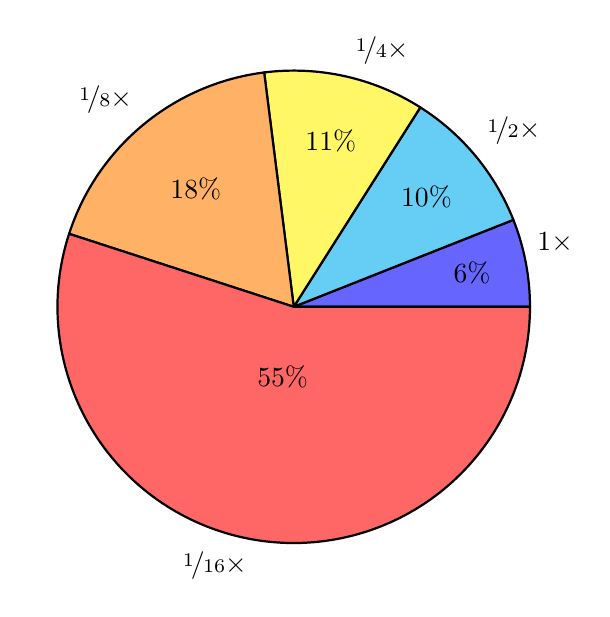
\begin{tikzpicture}
 
\pie{6/$1\times$,
    10/$\nicefrac{1}{2}\times$,
    11/$\nicefrac{1}{4}\times$,
    18/$\nicefrac{1}{8}\times$,
    55/$\nicefrac{1}{16}\times$}
 
\end{tikzpicture}} &
\resizebox{0.45\linewidth}{!}{
\begin{tabular}{@{}cl@{}}
\toprule
\multicolumn{1}{c}{\textbf{Model Capacity}} & \textbf{Annual Household Income} \\ \midrule
$\nicefrac{1}{16}\times$                 & $<\$75,000$           \\
$\nicefrac{1}{8}\times$                  & $\$75,000-\$100,000$           \\
$\nicefrac{1}{4}\times$                  & $\$100,000-\$150,000$          \\
$\nicefrac{1}{2}\times$                 & $\$150,000-\$200,000$          \\
$1\times$                                & $>\$200,000$     \\ \bottomrule
\vspace{5cm}
\end{tabular}} 
\end{tabular}
\vspace{-3.8cm}
    \caption{Mapping between real-world annual household income and model capacity.}
    \label{fig:my_label}
\end{figure}

\begin{table}[!htbp]
\centering
\caption{Experimental setup for Table \ref{tab:real_world_results} for CIFAR-10, CIFAR-100 \rebuttal{and Stack Overflow.} }
\label{tab:real_world_table_setup}
\resizebox{0.8\linewidth}{!}{%
\rebuttal{
\begin{tabular}{llccc} 
\toprule
\multicolumn{1}{c}{} &  & CIFAR-10 & CIFAR-100 & Stack Overflow \\ 
\cmidrule{1-5}
Local Epoch &  & 1 & 1 & 1 \\
Cohort SIze &  & 10 & 10 & 200 \\
Batch Size &  & 10 & 24 & 24 \\
Initial Learning Rate &  & 2.00E-04 & 1.00E-04 & 2.00E-04 \\
\multirow{2}{*}{Decay Schedule} & High Heterogeneity & 800, 1500 & 1000, 1500 & \multirow{2}{*}{600, 800} \\
 & Low Heterogeneity & 800, 1250 & 1000, 1500 &  \\
Decay Factor &  & 0.1 & 0.1 & 0.1 \\
\multirow{2}{*}{Communication Rounds~} & High Heterogeneity & 2500 & 3500 & \multirow{2}{*}{1200} \\
 & Low Heterogeneity & 2000 & 3500 &  \\
Optimizer &  & SGD & SGD & SGD \\
Momentum &  & 0.9 & 0.9 & 0.9 \\
Weight Decay &  & 5.00E-04 & 5.00E-04 & 5.00E-04 \\
\bottomrule
\end{tabular}
}
}
\end{table}






% \begin{figure}[htbp]
%     \centering
%     \resizebox{0.45\linewidth}{!}{
%     \begin{tikzpicture}
 
% \pie{6/$1\times$,
%     10/$\nicefrac{1}{2}\times$,
%     11/$\nicefrac{1}{4}\times$,
%     18/$\nicefrac{1}{8}\times$,
%     55/$\nicefrac{1}{16}\times$}
 
% \end{tikzpicture}}
% \resizebox{0.45\linewidth}{0.45\linewidth}{
% \begin{tabular}{@{}lc@{}}
% \toprule
% \multicolumn{1}{c}{\textbf{Model Size}} & \textbf{Annual Household Income} \\ \midrule
% $1\times$                               & \$\textless \$75,000\$           \\
% $\nicefrac{1}{2}\times$                 & \$\$75,000-\$100,000\$           \\
% $\nicefrac{1}{4}\times$                 & \$\$100,000-\$150,000\$          \\
% $\nicefrac{1}{8}\times$                 & \$\$150,000-\$200,000\$          \\
% $\nicefrac{1}{16}\times$                & \$ \$200,000\textgreater{}\$     \\ \bottomrule
% \end{tabular}}

%     \caption{Distribution of model capacities in real-world scenario proportioned according to income}
%     \label{fig:my_label}
% \end{figure}[]{}


\newpage
\subsection{Algorithm Pseudocodes}
\label{app:algorithm_pseudocode}
The pseudocodes for HeteroFL and Federated Dropout are given in Algorithms \ref{algo:HeteroFL} and \ref{algo:FedDropout} respectively. Their differences from \texttt{FedRolex} are marked using blue color. 

\begin{algorithm}[!h]
\caption{\textbf{HeteroFL}}
\label{algo:HeteroFL}
    \SetKwFunction{proc}{clientStep}
    \SetKwInOut{Input}{Input}
    \SetKwInOut{Output}{Output}

    % \underline{function Euclid} $(a,b)$\;
    Initialization ; $\theta^{(0)}$, $\mathcal{N}$\\
    \Input{$D_n\; \beta_n\; \forall n \in \mathcal{N}$, }
    \Output{$\theta^{J}$}
    \underline{Server Executes}\\    
    \For{$j\gets0$ \KwTo $J-1$}{
     Sample subset $\mathcal{M}$ from $\mathcal{N}$\\
     Broadcast $\theta^{(j)}_{m, [i\;;\; { 0, 1,\; ...\;\lfloor\beta_n K_i\rfloor-1}] } \forall i \;\text{and}\; m \in \mathcal{M}$\\
     \For{\textbf{each} client $m \in \mathcal{M}$}{
         \proc{$\theta^{(j)}_m$, $D_m$}
     }
     Aggregate $\theta^{(j+1)}_{[i, k]}$ according to Equation \eqref{eqn:theta_update} \\
    }
     \SetKwProg{step}{Subroutine}{}{}
     \step{\proc{$\theta^{(j)}_n$, $D_n$}}{
     $m_n \longleftarrow len(D_n)$\\
     \For{$k\gets0$ \KwTo $m_n$}{
        $\theta_n \longleftarrow \theta_n - \eta \nabla l(\theta_n; d_{n,k})$
        }
        return $\theta_n$
     }
\end{algorithm}

\begin{algorithm}[!h]
\caption{\textbf{Federated Dropout}}
\label{algo:FedDropout}
    \SetKwFunction{proc}{clientStep}
    \SetKwInOut{Input}{Input}
    \SetKwInOut{Output}{Output}

    % \underline{function Euclid} $(a,b)$\;
    Initialization ; $\theta^{(0)}$, $\mathcal{N}$\\
    \Input{$D_n\; \beta_n\; \forall n \in \mathcal{N}$, }
    \Output{$\theta^{J}$}
    \underline{Server Executes}\\    
    \For{$j\gets0$ \KwTo $J-1$}{
     Sample subset $\mathcal{M}$ from $\mathcal{N}$\\
     Broadcast $\theta^{(j)}_{m, [i\;;\; {k_1, ..., k_{\lfloor\beta_n K_i\rfloor}}] } \forall i  \;\text{and}\; m \in \mathcal{M}$\\
     \For{\textbf{each} client $m \in \mathcal{M}$}{
         \proc{$\theta^{(j)}_m$, $D_m$}
     }
     Aggregate $\theta^{(j+1)}_{[i, k]}$ according to Equation \eqref{eqn:theta_update}\\
    }
     \SetKwProg{step}{Subroutine}{}{}
     \step{\proc{$\theta^{(j)}_n$, $D_n$}}{
     $m_n \longleftarrow len(D_n)$\\
     \For{$k\gets0$ \KwTo $m_n$}{
        $\theta_n \longleftarrow \theta_n - \eta \nabla l(\theta_n; d_{n,k})$
        }
        return $\theta_n$
     }
\end{algorithm}



\end{document}
